%%%%%%%% ICML 2025 EXAMPLE LATEX SUBMISSION FILE %%%%%%%%%%%%%%%%%

\documentclass{article}

% Recommended, but optional, packages for figures and better typesetting:
\usepackage{microtype}
\usepackage{graphicx}
\usepackage{subfigure}
\usepackage{booktabs} % for professional tables

% hyperref makes hyperlinks in the resulting PDF.
% If your build breaks (sometimes temporarily if a hyperlink spans a page)
% please comment out the following usepackage line and replace
% \usepackage{icml2025} with \usepackage[nohyperref]{icml2025} above.
\usepackage{hyperref}


% Attempt to make hyperref and algorithmic work together better:
\newcommand{\theHalgorithm}{\arabic{algorithm}}

% Use the following line for the initial blind version submitted for review:
% \usepackage{icml2025}

% If accepted, instead use the following line for the camera-ready submission:
\usepackage[accepted]{icml2025}

% For theorems and such
\usepackage{amsmath}
\usepackage{amssymb}
\usepackage{mathtools}
\usepackage{amsthm}

% if you use cleveref..
\usepackage[capitalize,noabbrev]{cleveref}

%%%%%%%%%%%%%%%%%%%%%%%%%%%%%%%%
% THEOREMS
%%%%%%%%%%%%%%%%%%%%%%%%%%%%%%%%
\theoremstyle{plain}
\newtheorem{theorem}{Theorem}[section]
\newtheorem{proposition}[theorem]{Proposition}
\newtheorem{lemma}[theorem]{Lemma}
\newtheorem{corollary}[theorem]{Corollary}
\theoremstyle{definition}
\newtheorem{definition}[theorem]{Definition}
\newtheorem{assumption}[theorem]{Assumption}
\theoremstyle{remark}
\newtheorem{remark}[theorem]{Remark}

% Todonotes is useful during development; simply uncomment the next line
%    and comment out the line below the next line to turn off comments
%\usepackage[disable,textsize=tiny]{todonotes}
\usepackage[textsize=tiny]{todonotes}


% The \icmltitle you define below is probably too long as a header.
% Therefore, a short form for the running title is supplied here:
\icmltitlerunning{PieClam: A Universal Graph Autoencoder Based on Overlapping Inclusive and Exclusive Communities}

% OUR PACKAGES VV
\usepackage{afterpage}

\usepackage{amsmath}
\usepackage{amsthm}
\usepackage{pgfplots}
\usepackage{tikz}

\usepackage{subcaption}
\usepackage{lipsum}

\usepackage{xcolor}

%\usepackage{hyperref}

\usetikzlibrary{calc, angles, quotes}

%OUR PACKAGES ^^
%OUR DEFINITIONS VV

\newtheorem{claim}[theorem]{Claim}

\newcommand{\sumgraph}{\underset{n \in [N]}{\sum}}


\newcommand{\sumgraphm}{\underset{m \in [N]}{\sum}}


\def \sumgraphnotu {\underset{v \neq u }{ \sum}}

\def \sumgraphu {\underset{n\in [N]}{ \sum}}

\def \sumneighbors {\underset {m\in{\mathcal{N}(n)}}{\sum}}

\def \sumstrangers{\underset {m\notin{\mathcal{N}(n)}}{\sum}}

\newcommand{\flf}{\mathbf{f}_n^\top   \mathbf{L} \mathbf{f}_m}

\def \szemerdi{Szemerédi}

\newcommand{\ron}[1]{{{\textcolor{red}{\textbf{[Ron:} {#1}\textbf{]}}}}}
\newcommand{\dan}[1]{{{\textcolor{blue}{ {#1}\textbf{}}}}}
\usepackage{xcolor}

% OUR DEFINITIONS ^^




\begin{document}

\twocolumn[
\icmltitle{PieClam: A Universal Graph Autoencoder\\ Based on Overlapping Inclusive and Exclusive Communities}

% It is OKAY to include author information, even for blind
% submissions: the style file will automatically remove it for you
% unless you've provided the [accepted] option to the icml2025
% package.

% List of affiliations: The first argument should be a (short)
% identifier you will use later to specify author affiliations
% Academic affiliations should list Department, University, City, Region, Country
% Industry affiliations should list Company, City, Region, Country

% You can specify symbols, otherwise they are numbered in order.
% Ideally, you should not use this facility. Affiliations will be numbered
% in order of appearance and this is the preferred way.
\icmlsetsymbol{equal}{*}

\begin{icmlauthorlist}
\icmlauthor{Daniel Zilberg}{yyy}
\icmlauthor{Ron Levie}{yyy}
%\icmlauthor{}{sch}
%\icmlauthor{}{sch}
\end{icmlauthorlist}

\icmlaffiliation{yyy}{Faculty of Mathematics, Technion - Israel Institute of Technology, Haifa, Israel}
\icmlcorrespondingauthor{Daniel Zilberg}{dannyzilberg@gmail.com}
\icmlcorrespondingauthor{Ron Levie}{levieron@technion.ac.il}

% You may provide any keywords that you
% find helpful for describing your paper; these are used to populate
% the "keywords" metadata in the PDF but will not be shown in the document


\icmlkeywords{Machine Learning, ICML, Link Prediction, Anomaly Detection, Graph Neural Networks}

\vskip 0.3in
]

% this must go after the closing bracket ] following \twocolumn[ ...

% This command actually creates the footnote in the first column
% listing the affiliations and the copyright notice.
% The command takes one argument, which is text to display at the start of the footnote.
% The \icmlEqualContribution command is standard text for equal contribution.
% Remove it (just {}) if you do not need this facility.

%\printAffiliationsAndNotice{}  % leave blank if no need to mention equal contribution
\printAffiliationsAndNotice{}
%\printAffiliationsAndNotice{\icmlEqualContribution} % otherwise use the standard text.

\begin{abstract}
%We propose PieClam (Prior Inclusive Exclusive Cluster Affiliation Model): a probabilistic graph model for representing any graph as overlapping  generalized communities.  Our method can be interpreted as a graph autoencoder: nodes are embedded into a code space by an algorithm that maximizes the log-likelihood of the decoded graph, given the input graph. PieClam is a community affiliation model that extends well-known methods like BigClam in two main manners. First, instead of the decoder being defined via pairwise interactions between the nodes in the code space, we also incorporate a learned prior on the distribution of nodes in the code space, turning our method into a graph generative model. Secondly, we generalize the notion of communities by allowing not only sets of nodes with strong connectivity, which we call inclusive communities, but also sets of nodes with strong disconnection, which we call exclusive communities.  To model both types of communities, we propose a new type of decoder based the Lorentz inner product, which we prove to be much more expressive than standard decoders based on standard inner products or norm distances. By introducing a new graph similarity measure, that we call the log cut distance, we show that PieClam is a universal autoencoder, able to uniformly approximately reconstruct any graph. Our method is shown to obtain competitive performance in graph anomaly detection benchmarks.



%\dan{They say this should be cut down to 4-6 sentences...}

%\[\]


We propose PieClam (Prior Inclusive Exclusive Cluster Affiliation Model): a graph autoencoder, where nodes are embedded into a code space by an algorithm that maximizes the log-likelihood of the decoded graph. PieClam is a community affiliation model that extends well-known methods like BigClam in two main manners. First, instead of the decoder being defined via pairwise interactions between the nodes in the code space, we also incorporate a learned prior on the distribution of nodes in the code space, turning our method into a graph generative model. Secondly, we generalize the notion of communities by allowing not only sets of nodes with strong connectivity, which we call inclusive communities, but also sets of nodes with strong disconnection, which we call exclusive communities. By introducing a new graph similarity measure, called the log cut distance, we show that PieClam is a universal autoencoder, able to uniformly approximately reconstruct any graph. Our method is shown to obtain competitive performance in graph anomaly detection and link prediction benchmarks.

\end{abstract}





\section{Introduction}

In recent years, considerable research has concentrated on graph representation learning, aiming to develop vector representations for graph entities, including nodes, edges, and subgraphs \cite{hamilton2017representation,GRL_survet2020}. In graph autoencoders, e.g.,  \cite{kipf2016variational,grover2019graphite,JMLR:v21:19-671,mehta2019stochastic}, the vertices of a graph are embedded in a code space, where edges are inferred from the locations of the vertices in this space. Encoding graphs into a standard space has a number of advantages. While different graphs can have different sizes and topologies, the code space is fixed with a fixed dimension. This helps when  learning downstream tasks, where the representation of the graph in the code space can be processed. For example, in link prediction, one infers unknown edges by defining \cite{kipf2016variational} or learning \cite{kumar2020linkreview} a function that takes pairs of nodes in the code space and predicts if there is an edge between them. In anomaly detection, one defines \cite{ding2019dominant,fan2020anomalydae} or learns \cite{chen2020gaan,ding2021aegis}  a function that takes the representation of a node and its neighborhood and predicts if this node is normal or an anomaly. In graph and node classification, the graph is represented in the code space, and one learns a model that predicts from this representation the classes of the nodes or of the graph \cite{GCN,MPNN}. %\ron{references. Basically MPNNs,GNNs. Cite surveys and books.}. 

\paragraph{Our Contribution.} In this paper, we derive a new graph autoencoder from a statistical model of graphs. In our model, similarly to Stochastic Block Models (SBM) \cite{nowicki2001estimation,lee2019review} and community-based statistical models  \cite{airoldi2008mixed,yang2013BigClam}, graphs are generated from a combination of intersecting communities/cliques. Namely, each node belongs to a different subset of a predefined set of communities, and the affiliations of the nodes to the different communities determine the probabilities of the edges of the graph. Here, the estimation of the community affiliations is seen as an encoder of graphs to a  \emph{community affiliation space}, and the computation of the corresponding edge probabilities is seen as a decoder. As opposed to past works, we consider two types of \emph{generalized communities}. First, standard \emph{inclusive communities}, where any two nodes in the same community are likely to be connected. Second, we propose \emph{exclusive communities}, where belonging to the same community reduces the probability of nodes being connected. 

For illustration, consider a social network of employers/recruiters and employees/job-seekers. Such a network has roughly bipartite components, where job-seekers do not tend to connect to other seekers, and employers do not connect to other employers, but employers and seekers of the same subsector tend to connect. Hence, inclusive communities for such a graph can correspond to job titles or subsectors, and exclusive communities can correspond to sets of job-seekers and sets of employees from the same sector. For example, while the inclusive community of \emph{product management} will tend to connect all employers and specialists of product management to a ``clique-like'' community, the two exclusive communities of employers and of specialists of product management will each tend to delete the links between pairs of employers and between pairs of employees, creating a bipartite structure.

To formalize the above ideas, we propose the \emph{Prior Inclusive Exclusive Cluster Affiliation Model (PieClam)}. This model represents graphs as overlapping inclusive and exclusive communities. In addition to embedding the nodes of a given graph in the community code space, our model also learns a prior on the code space, so new graphs can be generated from the learned model. This makes PieClam a graph generative model, like, e.g.,  \cite{kipf2016variational,grover2019graphite,JMLR:v21:19-671,mehta2019stochastic,sun2019vgraph}. 

To model both types of communities, we propose a new type of decoder based on the \emph{Lorentz inner product}, in which case the code space is typically called a \emph{pseudo Euclidean space} \cite{greub1963pseudo}. The addition of exclusive communities in our model is not merely aimed at improving it heuristically for special graphs like social networks. Rather, we prove in Theorems \ref{thm:IEUniversality} and \ref{thm:IEUniversality2} that using exclusive communities (via the Lorentz inner product) makes our model universal, namely, able to approximate with a fixed budget of parameters any graph. This is in contrast to standard decoders based on merely inclusive communities, which we show are unable to represent many graphs. %In contrast, we prove that ou PieClam, based on the Lorentz inner product, can approximately represent any graph, of any size and topology, with a fixed limited budget of parameters.  

To formalize this universality property, we propose a new similarity measure between graphs with edge probabilities, that we call the \emph{log cut distance}. We formalize the universality of our model as follows: one can choose the dimension of the code space (the number of communities)  a priori, and guarantee that any graph of any size and topology can be approximated up to small log cut distance by decoding points from this fixed space. We show that other related decoders do not satisfy this universality property. 

In Section \ref{Experiments} we support our construction with experiments, where our models achieve competitive performance with respect to state of the art.
%We first conduct some toy experiments that illustrate the merits of our method.
First, we use PieClam to perform graph anomaly detection. Here, PieClam learns a probabilistic model given graph, and this model can be used for inspecting the probabilities of different nodes in this graph: nodes with low probabilities are deemed to be anomalies.  Then, we use PieClam to predict edges in link prediction benchmarks.


%
%Our method is shown to obtain competitive performance in graph anomaly detection benchmarks.


Appendix \ref{Extended Related Work} has 
%offers
an extended discussion on related work.

\section{Community Affiliation Models With Prior}

 %Hence, after introducing basic notations, we start with a detailed exposition of BigClam, before introducing our novel constructions.


\subsection{Notations}
\label{def:notations}
We denote by $\mathbb{R}_+$ the non-negative real numbers. We denote ``and'' by $\wedge$.
We denote matrices as boldface capital letter $\mathbf{B}=\{b_{n,m}\}_{n,m}$, vectors as boldface lowercase letters $\mathbf{b}=\{b_n\}_n$,  and scalars as  lowercase letters $b$. Vectors $\mathbf{b}\in\mathbb{R}^N$ are always column vectors. %, and their transpose $\mathbf{b}^{\top }$ row vectors. 
 The rows of a matrix $\mathbf{B}\in\mathbb{R}^{N\times C}$ are denoted by the same letter in lowercase $\mathbf{b}_n^{\top }$, where $\mathbf{b}_n\in\mathbb{R}^C$, where we write in short $\mathbf{b}_n^{\top }\in\mathbb{R}^C$. A diagonal matrix $\mathbf{D}\in\mathbb{R}^{N\times N}$ with diagonal entries $\mathbf{d}$ is denoted by ${\rm diag}(\mathbf{d})={\rm diag}(d_1,\ldots, d_N)$.  The $\ell^2$ norm of a vector $\mathbf{b} \in \mathbb{R}^N$ is defined to be $\|\mathbf{b}\| = (\sum_{n=1}^Nb_n^2)^{1/2}$. 

A graph is denoted by $G=([N],E,\mathbf{A})$, where $[N]=\{1,\ldots, N\}$ is the set of $N$ nodes,  $E\subseteq [N]\times[N]$ is the set of edges, and $\mathbf{A}\in \{0,1\}^{N\times N}$ is the adjacency matrix. For weighted graphs, $\mathbf{A}\in[0,1]^{N\times N}$, where $a_{n,m}$ is the edge weight of $(n,m)$.
In this work we focus on undirected graphs, for which $(m,n)\in E \Leftrightarrow (n,m)\in E$, and $\mathbf{A}=\mathbf{A}^{\top }$.  
%
Any pair $(n, m)\in [N]\times[N]$ is called a \emph{dyad}.
The neighborhood of a node $n\in[N]$ is  $\mathcal{N}(n)  = \{m \in [N] \mid (m,n) \in E\}$.
 A graph-signal is a graph with node features  $G=([N],E,\mathbf{A},\mathbf{X})$ where $\mathbf{X}=\{\mathbf{x}_n^{\top }\}_{n=1}^N\in \mathbb{R}^{N\times D}$, $\mathbf{x}_n\in\mathbb{R}^D$, and $D$ is called the feature dimension. 
A random graph is a graph-valued random variable. Given a random graph with nodes $[N]$, 
 we denote the event $(n,m)\in E$ by  $n\sim m$, and the event $(n,m)\notin E$ by $\neg (n\sim m)$.  
 %
%
A graph is bipartite if its vertex set $[N]$ can be partitioned into two disjoint sets $\mathcal{U}$ and $\mathcal{V}$, with  $\mathcal{U}\cup\mathcal{V}=[N]$, such that every edge has one endpoint in $\mathcal{U}$ and the other in $\mathcal{V}$. 
%In a complete bipartite graph, all of the nodes in $U$ are connected to all of the nodes in $W$ and there are no connections within the sets.

%In other words, a bipartite graph can be divided into two sets of nodes where each set connects to the other set but not within itself. 


\subsection{BigClam}
\label{sec:BigClam}
%\textcolor{red}{Explain the method. Introduce terms that we will use: affiliation space, dyad probability, etc (or maybe some of these belong in the previous chapter)}

%Since our model extends BigClam \cite{Overlapping2012}, let us start with introducing this model in detail. 
 Our model PieClam is best understood as an extension of the BigClam model \cite{Overlapping2012}. The code space in BigClam is $\mathbb{R}_+^C$, where each axis is interpreted as a community.  Each entry $f^c$ of a point $\mathbf{f}=(f^1,\ldots,f^C)\in\mathbb{R}_+^C$ is interpreted as how much the point belongs to community $c$, where $0$ means ``not included in $c$'' and $1$ ``included.'' In this paper we  call $\mathbb{R}_+^C$ \emph{the affiliation space (AS)}, and call any point in the affiliation space an \emph{affiliation feature (AF)}.

BigClam is a model where a simple random graph is decoded from a sequence of AFs $\mathbf{F}= \{\mathbf{f}_n=(f_n^1,\ldots,f_n^C)\}_{n=1}^N$ in the AS. For each pair of nodes $n\neq m\in[N]$, the probability of the event $\neg (n\sim m)$ (no edge between $n$ and $m$), given their amount of membership in the same community $c$, is defined to be
\[
%\label{eqn:poisson}
P(\neg (n\sim m)|f^c_n, f^c_m) = e^{-f^c_n f^c_m}.
\]
BigClam makes two assumptions of independence. First, the membership in one community does not affect the membership in another community. Hence,
\begin{equation}
\label{eq:ClamEdge}
    P(\neg (n\sim m))|\mathbf{F})=P(\neg (n\sim m))|\mathbf{f}_n, \mathbf{f}_m)=e^{-\mathbf{f}_n^{\top }\mathbf{f}_m},
\end{equation}
\[P(n\sim m)|\mathbf{F})=P(n\sim m|\mathbf{f}_n, \mathbf{f}_m)=1-e^{-\mathbf{f}_n^{\top }\mathbf{f}_m}.\]
Due to this formula, BigClam is a so called \emph{Bernoulli-Poisson model} 
(see Appendix \ref{Stochastic block models}  for more details).
The second assumption is that the events of having an edge between different pairs of nodes are independent.  As a result, the probability of the entire graph $([N],E)$ conditioned on the AFs $\mathbf{F}$ is
%\textcolor{cyan}{this formula is already given in the previous section,}
\begingroup
\begin{equation}
\footnotesize
\begin{aligned}
   &  P(E|\mathbf{F}) =\\
   &  \prod_{n \in [N]}\Bigg(
        \sqrt{\prod_{m \in \mathcal{N}(n)}P( n\sim m|\mathbf{F})\prod_{m \notin \mathcal{N}(n)} P(\neg (n\sim m)|\mathbf{F})}\Bigg)
\end{aligned}
\label{eqn:clam_prob}
\end{equation}
\endgroup
Here, the square root is taken because the product considers each edge twice, and all sums are over $m\neq n$.

BigClam consists of a decoder, decoding from the AFs $\mathbf{F}$ the random graph $G(\mathbf{F})$ with node set $[N]$ and independent Bernoulli distributed edges with probabilities $\mathbf{P}=\{P(n\sim m|\mathbf{f}_n, \mathbf{f}_m)\}_{n,m=1}^N$.

From the encoding side, given a simple graph $([N],E)$, BigClam encodes the graph into the affiliation space by maximizing the log likelihood with respect to the AFs $\mathbf{F}$
\begingroup
\footnotesize
\begin{align}
\label{eqn:naiveloss}
     l(\mathbf{F}) &= \frac{1}{2}\sumgraph \Big(\sumneighbors{}{\log(1-e^{-\mathbf{f}_n^{\top } \mathbf{f}_m})} - 
 \sumstrangers{\mathbf{f}_n^{\top } \mathbf{f}_m}\Big),
 \end{align}
 \endgroup
where all sums are over $m\neq n$. BigClam is optimized by gradient descent, with update at iteration $i$
    \begin{align}
    \label{eqn:vanilla_optimization}
    \mathbf{F}^{(i+1)} = \mathbf{F}^{(i)} + \delta\nabla_{\mathbf{F}}l({\mathbf{F}}^{(i)}),
    \end{align}
for some learning rate $\delta>0$.
In order to implement the above iteration with $O(|E|)$ operations at each step, instead of $O(N^2)$, the loss can be rearranged as
\begingroup
\begin{equation}
\footnotesize
\begin{aligned}
\label{eqn:comp_loss}
   &  2l(\mathbf{F})=\\
   & \sumgraphu \Big(\sumneighbors{\log(e^{\mathbf{f}_n^{\top } \mathbf{f}_n} - 1)}  - \mathbf{f}_n^\top {\sumgraph{\mathbf{f}_m}} + \|\mathbf{f}_n\|^2\Big).
\end{aligned}
\end{equation}
\endgroup
The gradient of the loss is now
\begin{align}
\label{eqn:BCupdate}
    % \nabla_{F_u}l = 
    % \sumneighbors{F_v \frac{e^{\inr[F_u]{F_v}}}{e^{\inr[F_u]{F_v}-1}}} - \sumgraph{F_v} + F_u \\
    \nabla_{\mathbf{f}_n}l = 
    \sumneighbors{\mathbf{f}_m \big(1-e^{-\mathbf{f}_n^\top  \mathbf{f}_m}
    \big)^{-1}} - \sumgraph{\mathbf{f}_m} + \mathbf{f}_n .
\end{align}
Since the global term needs to be calculated only once, the number of operations is  $O(|E|)$ instead of $O(N^2)$.  

We observe that the optimization process is a message passing scheme.
Looking at the dynamics of the optimization process, we see that every node is pushed in the direction of a weighted average of all of its neighbors, and pushed in the opposite direction to the average of all of the nodes. The sum of both forces tends to drive communities towards the axes in the optimization dynamics.


\subsection{Inclusive-Exclusive Cluster Affiliation Model}


%\textcolor{red}{Motivate the construction of bipartites. The need to find a decoder that satisfy what is needed of bipartites: two sets well connected to each other but not to themselves.} \textcolor{cyan}{i defined it in "notations"}
%\textcolor{cyan}{not sure how deep i should go about this... tell me if showing for a full bipartite is not good enough}
%To see the limited expressivity of a decoder that is monotonic with the inner product between nodes (like BigClam), let us consider what an embedding of a bipartite (\ref{def:notations}\textcolor{cyan}{problem referencing to sections as there is no numbering in this format}) graph should look like for it to be decoded in the best way. The nodes of $U$ will have to be perpendicular to one another, each being aligned with all of the nodes in $W$, which must also be perpendicular to one another.\textcolor{cyan}{don't know how to prove this yet. it's easy to show if the nodes are in a cluster}    
%\textcolor{cyan}{...}
%\textcolor{red}{Define the IeClam model.}



%\[\]

The BigClam decoder has a limitation due to a  ``triangle inequality type'' behavior. Namely, suppose that we would like to construct two features $\mathbf{f}_1$ and $\mathbf{f_2}$ with strong connectivity to a third feature $\mathbf{f}_3$, and  we are limited by a fixed affiliation feature dimension $C$. A naive approach to achieve this would be to put $\mathbf{f}_1$ and $\mathbf{f_2}$ close to $\mathbf{f}_3$ so they have large inner products $\mathbf{f}_1^{\top }\mathbf{f}_3$ and $\mathbf{f}_2^{\top }\mathbf{f}_3$ . This would mean that $\mathbf{f}_1^{\top }\mathbf{f}_2$ would also be large, so $\mathbf{f}_1$ would be strongly connected to  $\mathbf{f}_2$ under the BigClam model. However, some graphs, like bipartite graphs, do not exhibit this triangle inequality type behavior. For a rigorous treatment, see Section \ref{BigClam is Not Universal} and Appendix \ref{Proof That BigClam Is Not Universal}.  Next, we build the \emph{IeClam} decoder, that allows decoding any graph, that can model bipartite components without being limited by a  triangle inequality-type behavior. 

Our \emph{Inclusive Exclusive Cluster Affiliation Model (IeClam)} can be extended from BigClam by replacing the inner product in the non-edge probability (\ref{eq:ClamEdge}) by the more expressive \emph{Lorentz inner product}, which does not enforce a triangle inequality-type behavior. 
For that, we extend the affiliation space (AS) to be $\mathbb{R}^{2C}$, with two types of communities. The first $C$ axes are called the \emph{inclusive communities}, and their corresponding features are called \emph{inclusive affiliation features (IAF)}, denoted by $\mathbf{t}\in\mathbb{R}^C$. The last $C$ axes are called the \emph{exclusive communities}, with \emph{exclusive affiliation features (EAF)}, denoted by $\mathbf{s} \in \mathbb{R}^C$.\footnote{More generally, one can define a different number of inclusive and exclusive communities.} We define the concatenated affiliation feature by $\mathbf{f} = (\mathbf{t},\mathbf{s})\in\mathbb{R}^{2C}$. Given a sequence of affiliation features  $\mathbf{F}=\{\mathbf{f}_n\}_{n=1}^N\in\mathbb{R}^{N\times 2C}$, IeClam defines the probability of a single edge by
\begin{equation}
\begin{split}
    P(n\sim m| \mathbf{f}_n,\mathbf{f}_m) & = 1-\exp\big({-\mathbf{t}_n^{\top } \mathbf{t}_m +  \mathbf{s}_n^{\top } \mathbf{s}_m}\big) \\  
   &  = 1-\exp\big({-\mathbf{f}_n^{\top } \mathbf{L} \mathbf{f}_m}\big),
    \label{eq:LorFeature}
    \end{split}
\end{equation}
where $\mathbf{L} = {\rm diag}(1,...1,-1,...-1)$. The bilinear form $(\mathbf{u},\mathbf{v})\mapsto \mathbf{u}^\top  \mathbf{L} \mathbf{v}$ is called the \emph{Lorentz inner product}, and has its roots in special relativity. See Appendix \ref{The Lorentz Inner Product} for more details on the Lorentz inner product. 

Note that $\mathbf{L}$ is not positive-definite, so it does not actually define an inner product. Moreover, $\mathbf{f}_n^\top  \mathbf{L} \mathbf{f}_m$ can be negative even if $\mathbf{f}_n,\mathbf{f}_m\in \mathbb{R}_+^C$. To guarantee that (\ref{eq:LorFeature}) defines a proper probability between $0$ and $1$, we limit the affiliation space as follows.  
%
\begin{definition}
  A \emph{cone of non-negativity} is a  subset $\mathcal{C}$ of $\mathbb{R}^{2C}$ such that every $\mathbf{f},\mathbf{g}\in \mathcal{C}$ satisfy
$\mathbf{f}^\top  \mathbf{L} \mathbf{g} \geq 0$.  
\end{definition}
If we limit the affiliation space to be a cone of non-negativity, then IeClam gives well defined edge probabilities in $[0,1]$.
In our experiments, we restrict ourselves to the following simple construction of a cone of non-negativity, noting that it is not the only possible construction. 
%
%For each $c\in[C]$, we take the direct product of axis $c$ with axis $C+c$, and denote it by $\mathcal{C}^c=\sim\mathbb{R}^2$. Given $\mathbf{f}\in\mathbf{C}^{2C}$, we call $(t^c,s^c)$ the entry of $\mathbf{f}$ in $\mathcal{C}^c$. 
\begin{definition}
 The \emph{pairwise cone} $\mathcal{T}^C$ is defined to be the set of affiliation features $\mathbf{f}=(\mathbf{t},\mathbf{s})\in\mathbb{R}^{2C}$ such that for every $c\in[C]$ we have $-t^c \leq s^c\leq t^c$.    
\end{definition}
It is easy to see that $\mathcal{T}^C$ is a cone of non-negativity. Indeed, for any $\mathbf{f}_1=(\mathbf{t}_1,\mathbf{s}_1), \mathbf{f}_2=(\mathbf{t}_2,\mathbf{s}_2) \in \mathcal{T}^C$,  we have  
 \[\forall c\in[C]: \quad  t_1^c t_2^c - s_1^c s_2^c \geq 0,\] so
\[\mathbf{f}_1^\top  \mathbf{L} \mathbf{f}_2 = \sum_{c=1}^C t_1^c t_2^c - s_1^c s_2^c \geq 0.\] 
%
%
As opposed to the BigClam decoder, the IeClam model can approximate a bipartite graph with a small number of communities. Namely, a bipartite graph with two (disjoint) sides $\mathcal{U},\mathcal{V}\subset[N]$ and constant probability for edges between $\mathcal{U}$ and $\mathcal{V}$ can be represented using $C=1$. Here,  all of the nodes in $\mathcal{U}$ are encoded to $(a,a)$,  and all of the nodes of $\mathcal{V}$ are encoded to $(a,-a)$, for some $a\geq 0$. This gives zero probability for edges within each part, and probability $1- e^{-2a^2}$ for edges between the parts. %1- e^{-2a^2}%\ron{now write the construction that approximates a full bipartite graph (where the probability of having a edge between any two nodes from opposite sides is a constant).}

\begin{remark}
    The above construction gives an interpretation for each pair of axes $(t^c,s^c)$ in $\mathcal{T}^C$ as a \emph{generalized community} which can model anything between a clique and a bipartite component.
\end{remark}

%for every $u \in U$ and  $w \in W$, a complete bipartite graph can be encoded using $\mathbf{f}_u = (a,a)$  and $\mathbf{f}_w = (a,-a)$, for some scalar $a\in \mathbb{R}/{0}$. In this construction, $P(u\sim w) = 1- e^{-2a^2}$ which goes to $1$ when $a \rightarrow \infty$, and $P(\neg(u_1\sim u_2)) = P(\neg(w_1\sim w_2)) = 0$ for all $u_1,u_2 \in U$ and $w_1, w_2 \in W$ . 

Given AFs $\mathbf{F}$ in a cone, IeClam is seen as a decoder, by decoding $\mathbf{F}$ into the random graph $G(\mathbf{F})$ with node set $[N]$ and independent Bernoulli distributed edges with probabilities $\mathbf{P}=\{P(n\sim m|\mathbf{f}_n, \mathbf{f}_m)\}_{n,m=1}^N$.

For affiliation features $\mathbf{F}\in \mathcal{T}^{C\times N}$, the probability of the graph $([N],E)$ given $\mathbf{F}$ of IeClam is
\begingroup
\footnotesize
\begin{equation}
\begin{aligned}
   &  P(E|\mathbf{F}) \\
   & = \prod_{n \in [N]}\Bigg(
        \sqrt{\prod_{m \in \mathcal{N}(n)}(1-e^{-\mathbf{f}_n^\top  \mathbf{L} \mathbf{f}_m})\prod_{m \notin \mathcal{N}(n)} e^{-\mathbf{f}_n^\top  \mathbf{L} \mathbf{f}_m}}\Bigg).
\end{aligned}
\label{eqn:IeClam_prob}
\end{equation}
\endgroup
Like BigClam, IeClam is optimized by maximizing the log likelihood with gradient descent
\begin{equation}
\begin{aligned}
   &  2 l(\mathbf{F}) =
    \\ &\sumgraphu \Big(\sumneighbors{}\log(1 - e^{-{\mathbf{f}_n}^\top  \mathbf{L} \mathbf{f}_m})  -   \sumstrangers{}  \mathbf{f}_n ^\top  \mathbf{L} \mathbf{f}_m\Big)
    \end{aligned}
\label{eqn:IeClam_loss}
\end{equation}
This loss can be efficiently implemented on sparse graphs, with $O(|E|)$ complexity, by the formulation
\begingroup
\begin{equation}
\footnotesize
\begin{aligned}
\label{eqn:loss_reparam_ie}
   &  2l(\mathbf{F})=\\
   & \sumgraphu \Big(\sumneighbors{\log(e^{\flf} - 1)}  - \mathbf{f}_n^\top  \mathbf{L}{\sumgraphm{\mathbf{f}_m}} + \mathbf{f}_n^\top  \mathbf{L}\mathbf{f}_n\Big).
\end{aligned}
\end{equation}
\endgroup
The gradient of the loss for node $n$ is
\begin{align}
\label{eqn:BCupdate_ie}
    \nabla_{\mathbf{f}_n}l = 
   \mathbf{L}\bigg( \sumneighbors{\mathbf{f}_m \big(1-e^{-\flf}
    \big)^{-1}} - \sumgraphm{\mathbf{f}_m} + \mathbf{f}_n \bigg).
\end{align}
Notice that all of the calculations are the same as BigClam, up to replacing the dot product by the Lorenz inner product. Hence, the optimization process  of IeClam is a message passing scheme, and equivariant to node re-indexing.
%We can see that any reconstruction achieved using BigClam with $C$ communities can also be achieved using IeClam with $2C$ IE communities. In practice, when graphs have strong inclusive connections, IeClam can preform worse than BigClam due to overfitting.

% \textcolor{cyan}{add an explanation for allowing the features in the time cone so that the product is non negative. nodes on opposide sides of the cone have a high probability of connecting, as well as features with high t and low s}
% We refer to $\mathbf{t}$ communities as "inclusive", since if the affiliation of two nodes to a $\mathbf{t}$ type community is of the same sign it increases the probability of connection. Similarly, if the affiliations of two nodes to an $\mathbf{s}$ community is of an opposite sign it increases the probability of connection.

% The inclusive-exclusice (IE) modification replaces the Hilbert code space with a version of the Minkowski space where there are the same amount of "time" coordinates as there are "space" coordinates \textcolor{cyan}{citation? i think from books you need to give the page}. 

% For the probability model to hold, we need the argument of the exponent to be positive. This was easy when there were only inclusive communities and indeed, BigClam was restricted to positive features To avoid divergence of the model. 

% In order to achieve positivity in the exponent argument we restrict the domain to pairs of "time-cones".
% \begin{definition}
%     For a node $n\in[N]$, a timecone is defined to be the pair $\mathbf{\tau}_n[i] = (t_n[i], s_n[i]) = (f_n[i], f_n[i+k])$  
% \end{definition}
% For all time cones we restrict $-t_n[i] \leq s_n[i] \leq t_n[i]$.
% The definition of timecones assures that the argument of the exponent is always non positive. Despite being a subset of ${\mathbf{f}_n}^\top  B \mathbf{f} \geq 0$, restriction of features to the timecones eases the computation time and breaks the symmetry of the initial IE definition, creating generalized communities which can be interpreted as each having an inclusive and exclusive part.

% In some cases, BigClam can still outperform IeClam as graphs can have a strong community structure that can be overfitted with IeClam.

\subsection{Community Affiliation Models With Prior}

%\textcolor{red}{Talk about the limit of BigClam and IeClam as generative models- no way to approximate different graphon this way.}
BigClam and IeClam are not  generative graph models. Indeed, these methods only fit a conditional probability of the graph, conditioned on the AF values, but the methods do not learn the probability of the AFs over the affiliation space. Hence, the total probability of $E\wedge\mathbf{F}$ is not defined. %If one was trying to generate a graph using only the features learned using this model, they could only either use the learned node features, or interpolate them in some way that is not rigorous. In the other direction, there is no option to obtain the probability of a test graph given a training graph, only by running the method again for the test graph.
%
%Therefore, neither of the models can be considered a generative graph model, as they do not provide a distribution over the AS.

%\textcolor{red}{Explain our solution - define a prior distribution in the affiliation space.}
To extend IeClam (and similarly BigClam) into probabilistic generative models, we define a prior probability distribution over the affiliation cone space $\mathcal{C}\subset \mathbb{R}^{2C}$, with probability density function $p:\mathbb{R}^{2C}\rightarrow [0,\infty)$ supported on $\mathcal{C}$. Using Bayes law, we now obtain the joint probability $P(E \wedge \mathbf{F})$ of the edges and community affiliation features  via the probability density function
\begin{align*}
    p(E ,\mathbf{F}) = P(E|\mathbf{F}) p(\mathbf{F}).
\end{align*}
We assume that the prior probabilities of all nodes are independent, namely,  
\[p(\mathbf{F}) = \underset{n\in [N]}{\prod} p(\mathbf{f}_n).\]
 Hence, the probability densities that a dyad $(n,m)$ is an edge or non-edge are
\[p(n\sim m, \mathbf{f_n}, \mathbf{f_m}) = p(\mathbf{f}_n)p(\mathbf{f}_m)(1 - e^{-{\mathbf{f}_n}^\top  \mathbf{L} {\mathbf{f}_m}}),\]
\[p(\neg(n\sim m), \mathbf{f_n}, \mathbf{f_m}) = p(\mathbf{f}_n)p(\mathbf{f}_m)e^{-{\mathbf{f}_n}^\top  \mathbf{L} {\mathbf{f}_m}}.\]
As before, we assume that the probabilities of different edges are independent, which gives
\begingroup
\scriptsize
\begin{equation}
\label{eqn:likelihood_prior}
\begin{aligned}
    &p(E, \mathbf{F}) =  \\ &\prod_{n \in [N]} p(\mathbf{f}_n)
        \sqrt{\prod_{m \in \mathcal{N}(n)}P(n\sim m|\mathbf{F}_m)\prod_{m \notin \mathcal{N}(n)}{P(\neg(n\sim m)|\mathbf{f}_n, \mathbf{f}_m)}
        }. 
 \end{aligned}
 \end{equation}
 \endgroup
Now, the log likelihood loss is
\begingroup
\begin{equation}
\footnotesize
\begin{aligned}
\label{eqn:loss_reparam_pie}
   &  l(\mathbf{F})= \sumgraphu \Bigg(\log(p(\mathbf{f}_n)) + \\
   & \quad  \frac{1}{2} \Big(\sumneighbors{\log(e^{\flf} - 1)}  -  \mathbf{f}_n^\top  \mathbf{L}{\sumgraphm{\mathbf{f}_m}} + \mathbf{f}_n^\top  \mathbf{L}\mathbf{f}_n \Big) \Bigg).
\end{aligned}
\end{equation}
\endgroup
We call this extension of IeClam PieClam (Prior Inclusive Exclusive Cluster Affiliation Model). We similarly extend BigClam to PClam (Prior Cluster Affiliation Model) by replacing $\mathbf{L}$ in (\ref{eqn:loss_reparam_pie}) with the identity matrix. 

Observe that the PieClam loss is similar to the IeClam loss, only with the addition of the prior acting as a per node regularization term. The prior attracts all nodes to areas of higher probability during the optimization dynamics. As before, the optimization process  of PieClam is a message passing scheme with $O(|E|)$ complexity, and is  equivariant to node re-indexing. Also, note that adding the prior to the Clam model only takes $O(|N|)$ complexity, which is lower than the complexity of the IeClam terms.

In order to sample from the above generative models, we first sample features $\{\mathbf{f}_n\}_{n\in [N]}$ according to $p$, and then connect them using either the BigClam or IeClam conditional probability.
%
To model the prior in practice, we use \emph{realNVP},  which is a \emph{normalizing flow} neural network model \cite{dinh2016density}. For more details on normalizing flows, see Appendix \ref{extended_sec:normflows}.



\paragraph{PieClam for graphs with node features.}
\label{sec:pieclam for graphs with node features}
%\textcolor{red}{Say that the prior maps to the direct product space of the affiliation space and the feature sapce.}

So far, we have used only the topology of the graph, not considering node features. 
We extend PieClam (and PClam) to graph-signals $([N], E, \mathbf{X})$ as follows. Concatenate the feature space of $\mathbf{X}$ to the affiliation space, and learn the prior on this combined space. This only affects the prior $p$. The conditional edge probabilities are  defined only in terms of the affiliation features, as before.

\section{Universality of PieClam and IeClam}

In this section, we define the universality of graph autoencoders, and prove that IeClam and PieClam are universal, while BigClam and PClam are not. The motivation behind the universality definition is that we would like to uniformly choose the dimension of the code space, such that every graph can be approximated by decoding some points in this fixed code space. Namely, we would like one \emph{universal} decoder that works for all graphs, as opposed to choosing the dimension of the code space depending on the graph.

\subsection{General Graph Autoencoders}

Next, we define a general decoder that defines edge probabilities  by operating on pairs of points in a code space. 

\begin{definition}
   A \emph{pairwaise decoder} over the code spaces $\mathbb{R}^M$ is a mapping $D_M:\mathbb{R}^{2M}\rightarrow[0,1]$. Given $N$ points in the code space $\mathbf{z}=\{z_n\in\mathbb{R}^M\}_{n=1}^N$, the decoded graph $G_N(\mathbf{z})$ is the weighted graph with adjacency matrix  
\[\mathbf{D}_M(\mathbf{z})=\big(D_M(z_n,z_k)\big)_{n,k=1}^N.\]
\end{definition}

Clam models are special cases of pairwise decoders.

%The pairwise decoders of of the Clam models involve a construction with an exponential, which cannot attain probability 1.

\subsection{Log Cut Distance}

Our definition of universality has the following form: for every error tolerance $\epsilon>0$, there is a choice of the dimension $M(\epsilon)$ of the code space such that every graph can be approximated up to error $\epsilon$ by decoding some points in this space. To formalize the ``up to error $\epsilon$'' statement, we present in this section a new graph similarity measure which we call the log cut distance.
Our construction is based on a well-known graph similarity measure called the cut norm.

\begin{definition}
  The \emph{cut norm} of a matrix $\mathbf{X}\in\mathbb{R}^{N\times N}$ is defined to be
    \begin{equation}
    \label{eq:GraphCutNorm0}  \|\mathbf{X}\|_{\square}:=\frac{1}{N^2}\sup_{\mathcal{U},\mathcal{V}\subset[N]}\Big|\sum_{i\in \mathcal{U}}\sum_{j\in \mathcal{V}}x_{i,j}\Big|.
\end{equation}  
\end{definition}
The \emph{cut metric} $\|\mathbf{A}-\mathbf{B} \|_{\square}$ between two adjacency matrices $\mathbf{A}$ and $\mathbf{B}$ is interpreted as the difference between the edge densities of $\mathbf{A}$ and $\mathbf{B}$ on the block $\mathcal{U}\times\mathcal{V}$ on which their edge densities are the most different.

The following graph similarity measure modifies the cut norm, making it appropriate for graphs with random edges over a fixed node set.
\begin{definition}
\label{def:KL1}
Given two random graphs over the nodes set $[N]$, with independently Bernoulli distributed edges with probabilities $\mathbf{P}=\{p_{n,m}\}_{n,m\in[N]}$ and $\mathbf{Q}=\{q_{n,m}\}_{n,m\in[N]}$ respectively, their \emph{log cut distance} is defined to be 
\begin{equation}
\footnotesize
    \begin{split}
       & D_{\square}(\mathbf{P} || \mathbf{Q}):=  \inf_{0< e,d\leq 1} \Bigg( e+d+ \\
       &  \quad \quad \  \frac{1}{N^2}\sup_{\mathcal{U},\mathcal{V}\subset[N]}\Big|\log\Big(\prod_{n\in \mathcal{U}}\prod_{m\in \mathcal{V}}
\frac{1-(1-e)p_{n,m}}{1-(1-d)q_{n,m}}\Big)\Big|\Bigg).
    \end{split}
    \label{eq:KL1}
\end{equation}
\end{definition}
The second term in (\ref{eq:KL1}) is the cut distance $\| \tilde{\mathbf{P}}-\tilde{\mathbf{Q}}\|_{\square}$ between the matrix $\tilde{\mathbf{P}}$ with entries 
\[\tilde{p}_{n,m}=-\log(1-(1-e)p_{n,m})\]
and the matrix $\tilde{\mathbf{Q}}$
 with entries 
 \[\tilde{q}_{n,m}=-\log(1-(1-d)q_{n,m}).\] Namely, the cut distance between the log likelihoods of non-edges. The parameters $e$ and $d$ make the $[0,1]$-valued probabilities valid inputs to the log. The goal of $e,d$ is to regularize the probability of the edges, where higher regularization is penalized via the additive term $e+d$. % in (\ref{eq:KL1}).

%\ron{Change to cut relative entropy? Or something else? since we don't have the probability times log probability... Change it here an in the abstract to log cut distance?}
% The above similarity measure is related  to the \emph{Kullback-Leibler (KL) divergence}. Namely, 
For each choice of a cut $\mathcal{U},\mathcal{V}\subset[N]$,  the term
 \begin{equation}
 \label{eq:KL2}
     \frac{1}{N^2}\log\Big(\prod_{n\in \mathcal{U}}\prod_{m\in \mathcal{V}}
\frac{1-(1-e)p_{n,m}}{1-(1-d)q_{n,m}}\Big)
 \end{equation}
is somewhat similar in structure to an un-normalized KL divergence, or distance of log likelihoods, between the non-edge probabilies of the graphs $\mathbf{P}$ and $\mathbf{Q}$ over the dyads between  $\mathcal{U}$ and $\mathcal{V}$. Here, ``un-normalized'' means that the dyads are drawn  uniformly with probabilities $1/N^2$, but the sum of probabilities is $|\mathcal{U}|\cdot|\mathcal{V}|/N^2$ and not 1. The un-normalized uniform distribution discourages the supremum inside the definition of $D_{\square}$ from choosing small blocks for maximizing (\ref{eq:KL2}). Note that normalized uniform distributions would lead $D_{\square}$ to choose  small blocks, which do not reflect meaningful empirical estimates of the edge statistics (the edge densities of small blocks would not be interpretable as expected number of edges). To conclude, $D_{\square}(\mathbf{P} || \mathbf{Q})$ is interpreted as the maximal divergence between $\mathbf{P}$ and $\mathbf{Q}$ over all blocks, up to the best regularizers. % $e,d$.

In our analysis we compute the log cut distance between the random decoded graph $\mathbf{P}$ and the deterministic target graph $\mathbf{A}$. While $\mathbf{A}$ has edge probabilities in $\{0,1\}$, $\mathbf{P}$ has edge probabilities in $[0,1)$ for Clam models. Therefore, we only require regularization  for $\mathbf{A}$. We hence consider the following modified version of Definition \ref{def:KL1}.
\begin{definition}
\label{def:KL2}
Given an unweighted graph with adjacency matrix $\mathbf{A}\in\{0,1\}^{N\times N}$ and a random graph over the nodes set $[N]$, with independently Bernoulli distributed edges with probabilities $\mathbf{P}=\{0\leq p_{n,m}<1\}_{n,m\in[N]}$, the \emph{log cut distance} between $\mathbf{P}$ and $\mathbf{A}$ is defined to be
    \[\footnotesize
    \begin{split}
    & D_{\square}(\mathbf{P} || \mathbf{A}):= \\
    & \inf_{0< d\leq1} \Bigg( d+ \frac{1}{N^2}\sup_{\mathcal{U},\mathcal{V}\subset[N]}\Big|\log\Big(\prod_{n\in \mathcal{U}}\prod_{m\in \mathcal{V}}
\frac{1-p_{n,m}}{1-(1-d)a_{n,m}}\Big)\Big|\Bigg).
\end{split}\]
\end{definition}

Lastly, in case both $\mathbf{P}$ and $\mathbf{Q}$ are $[0,1)$-valued, a simple version of the log cut distance is (\ref{eq:KL1}) with the choice $e=d=0$, namely,
 \[D^0_{\square}(\mathbf{P} || \mathbf{Q}):=\]
 \begin{equation}
    \label{eq:KL3}
         \frac{1}{N^2}\sup_{\mathcal{U},\mathcal{V}\subset[N]}\Big|\log\Big(\prod_{n\in \mathcal{U}}\prod_{m\in \mathcal{V}}
\frac{1-p_{n,m}}{1-q_{n,m}}\Big)\Big|.
    \end{equation}



\subsection{Universal Graph Autoencoders}

We are now ready to define the universality of general pairwise autoencoders. Motivated by the fact that a Clam autoencoder is actually a family of autoencoders, parameterized by the number of communities, we also define general pairwise decoders as families.

\begin{definition}
    A family of code spaces $\mathbb{R}^M$ and corresponding pairwaise decoders $D_M:\mathbb{R}^{2M}\rightarrow[0,1]$, parametrized by $M\in\mathbb{N}$, is called  \emph{universal} if for every $\epsilon>0$ there is $M\in\mathbb{N}$ (which depends only on $\epsilon$) such that for every $N\in\mathbb{N}$ and every graph  with adjacency matrix $\mathbf{A}$ and $N$ nodes there are $N$ points in the code space $\{z_n\in\mathbb{R}^M\}_{n=1}^N$ such that 
     $D_{\square}(\mathbf{D}_M(\mathbf{z}) || \mathbf{A}) <\epsilon$.  
\end{definition}

\subsection{BigClam and PClam are Not Universal}
\label{BigClam is Not Universal}

We now show that BigClam (and hence also PClam) is not a universal autoencoder since it cannot approximate bipartite graphs.
Consider the bipartite graph $\mathbf{B}$ with $N$ nodes at each part, and probability $1-e^{-a^2}$ for an edge between the two parts, and $0$ within each part. 
Since in this case all probabilities are less than 1, we can use (\ref{eq:KL3}) as the definition of the log cut distance. The analysis for Definition \ref{def:KL2} extends naturally.

Let $\mathbf{P}$ be a decoded BigClam graph. 
We show that there is no way to make $D^0_{\square}(\mathbf{P} || \mathbf{Q})$ small by choosing the dimension $C$ uniformly with respect to $N$. In fact, we will show BigClam cannot approximate a bipartite graph at all.\footnote{In Appendix \ref{BigClam With No Self Loops Approximating Bipartites} we show that one can approximate a bipartite graph of $2N$ nodes using $C=N^2$ classes in BigClam if the model ignores self-loops.} 

\begin{claim}
\label{claim:Clam_bi}
    Under the above construction, 
    \[D^0_{\square}(\mathbf{P} || \mathbf{B}) \geq \frac{a^2}{16}.\]
    As a result, BigClam is not a universal autoencoder.
\end{claim}
The proof is given in Appendix \ref{Proof That BigClam Is Not Universal}.
We note that one can similarly show that BigClam is not universal also with respect to the log cut distance of Definition \ref{def:KL2}.


\subsection{Universality of IeClam and PieClam}
We are now ready to show that IeClam (and hence also PieClam) is a universal autoencoder. The proofs of the following two theorems are in Appendix \ref{Proof of the Universality of PieClam} and \ref{Proof of the Universality of IeClam in a Cone of Non-negativity}.

We give two versions for the universality result. The first is without a cone restriction, and requires a relatively small number of communities for the given error tolerance. The corresponding decoder produces edge weights that can be negative. The second theorem is restricted to the pairwise cone of non-negativity, and has pessimistic  asymptotics for the required number of communities given an error tolerance. The second decoder is guaranteed to produce proper edge probabilities in $[0,1)$.



\begin{theorem}
\label{thm:IEUniversality}
    For every epsilon $\epsilon>0$, every $N\in\mathbb{N}$, and every adjacency matrix $\mathbf{A}\in[0,1]^{N\times N}$, there are $N$ affiliation features $\mathbf{F}\in \mathbb{R}^{2K}$ of dimension  $K=-9\log(\epsilon/2)^2/\epsilon^2$ such that the corresponding IeClam model $\mathbf{P}=\{P(n\sim m|\mathbf{f}_n, \mathbf{f}_m)\}_{n,m=1}^N$ satisfies 
     $D_{\square}(\mathbf{P} || \mathbf{A}) <\epsilon$.  
    Here, the log cut distance is from Definition \ref{def:KL2}.
    As a result, 
    IeClam and PieClam are universal autoencoders with code space $\mathbb{R}^{2K}$.
\end{theorem}

\begin{theorem}
\label{thm:IEUniversality2}
    For every epsilon $\epsilon>0$, every $N\in\mathbb{N}$, and every adjacency matrix $\mathbf{A}\in[0,1]^{N\times N}$, there are $N$ affiliation features $\mathbf{F}$ in the cone of pairwise non-negativity  $\mathcal{T}^C\subset \mathbb{R}^{2C}$ of dimension  $C=2^{4\lceil -\log(\epsilon/2)^2/\epsilon^2\rceil}$  such that the corresponding IeClam model $\mathbf{P}=\{P(n\sim m|\mathbf{f}_n, \mathbf{f}_m)\}_{n,m=1}^N$ satisfies 
     $D_{\square}(\mathbf{P} || \mathbf{A}) <\epsilon$.  
    Here, the log cut distance is from Definition \ref{def:KL2}.
    As a result, 
    IeClam and PieClam are universal autoencoders with code space $\mathcal{T}^C$.
\end{theorem}

\subsection{Log cut distance and maximum likelihood}

It is well known that it is NP hard to compute cut distance \cite{CutNP1,CutNP2}, %[Noga Alon and Assaf Naor. Approximating the cut-norm via grothendieck’s inequality.SIAM, 2006, Jiří Rohn. Computing the norm a infinity to 1 is np-hard. Linear and Multilinear Algebra,2000], 
and hence also log cut distance. Instead, we observe that maximizing log likelihood, which is efficiently implemented with gradient ascent, leads to a small log cut distance in practice. See Figure  \ref{fig:222}.
\begin{figure}[H]        
\centering
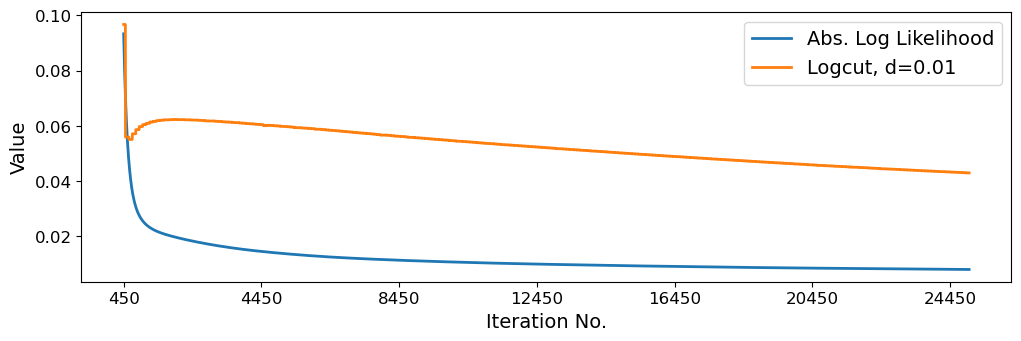
\includegraphics[width=0.46\textwidth]{images/distance/distance_squirrel_ieclam.png}
    \caption{The value of log cut vs. the absolute value of log likelihood along the optimization of IeClam on Squirrel. When log likelihood is optimized, log cut distance decreases.}
        \label{fig:222}
\end{figure}



%\ron{\Large ADD} 
%\ron{make a plot with the best d for each dataset and several dataset for which the log cut goes down. We show this result for the datasets Photo, Elliptic, Texas and a synthetic off diagonal SBM.}

\section{Experiments}

All of the experiments were run on Nvidia GeForce RTX 4090 and Nvidia L40 GPUs.\footnote{
Our code can be found in:  \url{https://github.com/danizil/PieClam} }

\dan{For modeling the prior we used a RealNVP \cite{dinh2016density} model with $32$ coupling blocks, each consisting of $2$ layer MLPs with a hidden dimension of $64$ and weight decay of $0.1$. This architecture was used across all experiments.}

\label{Experiments}

%\textcolor{cyan}{should also write about the fact that the model works well without node features. (actually, on the real anomalies, the features almost don't matter)}

%We conduct experiments that showcase and support our theoretical constructions.

% \subsection{Reconstructing Synthetic Priors}
% \label{sec:reconstruction_prior}

% We consider a ground-truth synthetic prior $p:\mathbb{R}^C\rightarrow[0,\infty)$ in PClam. %, modeled via a realNVP normalizing flow \cite{dinh2016density}. 
% We sample $N=500$ points from the prior, decode the corresponding PClam graph, and sample a simple graph from the random Bernoulli edges. Then, given these sampled graph, we fit to it a PClam and  model. In Figure~\ref{fig:prior_reconstruction} we compare the ground-truth prior to the reconstructed prior. We observe that even though our method is unsupervised, it still manages to capture the prior qualitatively well. More details are given in Appendix \ref{Extended Details on Experiments}.

% \begin{figure}[!t]
%     \begin{minipage}{0.3\columnwidth}
%         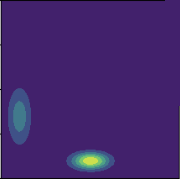
\includegraphics[width=\textwidth]{images/synthetic_2d/two_gaussians/r.png}
        
%     \end{minipage}\hfill
%     \begin{minipage}{0.3\columnwidth}
%         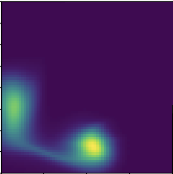
\includegraphics[width=\textwidth]{images/synthetic_2d/two_gaussians/c.png}
        
%     \end{minipage}\hfill
%     \begin{minipage}{0.3\columnwidth}
%         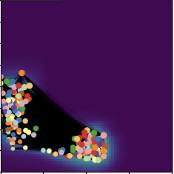
\includegraphics[width=\textwidth]{images/synthetic_2d/two_gaussians/ppp.png}
        
%     \end{minipage}
%     \caption{Left to right: Synthetic prior in an affiliation space of two inclusive communities.  Reconstructed prior by PClam with normalizing flow.  Reconstructed affiliation features by PClam.}
%     \label{fig:prior_reconstruction}
% \end{figure}

%\lipsum[1-5] % Dummy text
%\begingroup
%\color{blue}
\subsection{Reconstructing Synthetic Priors}
\label{sec:reconstruction_prior}
We consider a ground-truth synthetic prior $p$. % $p:\mathcal{T}^1\rightarrow[0,\infty)$. %, modeled via a realNVP normalizing flow \cite{dinh2016density}. 
We sample $N=500$ points from $p$, decode the corresponding PieClam graph, and sample a simple graph from the random Bernoulli edges.
Then, using the sampled graph as the target for the PieClam optimization, we fit PieClam on $\mathcal{T}^1$.
The results are shown in Figure \ref{fig:prior and sampled}. We observe that the algorithm  reconstructs both the positions of the nodes in the affiliation space and the original prior qualitatively well. 
Additional Experiments and results are given in Appendix \ref{app_sec:reconstruction_prior}.


\begin{figure}[H]        
\centering
\begin{minipage}{0.99\columnwidth}
        
\includegraphics[width=0.47\textwidth]{images/synthetic_2d/circle/circle_ie_gt.png} 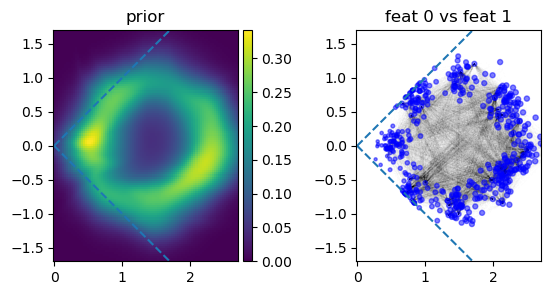
\includegraphics[width=0.52\textwidth]{images/synthetic_2d/circle/pieclam_circ_reconstruct_edges.png}
        \end{minipage} 
        
        \caption{Left to right:  Ground truth synthetic prior in $\mathcal{T}^1$; Graph sampled from the prior; Reconstructed prior via PieClam; Reconstructed nodes via PieClam. }
        \label{fig:prior and sampled}
\end{figure}




        


%\begin{figure}[H]
%\centering
%    \begin{minipage}{0.3\textwidth}
%        \centering
        %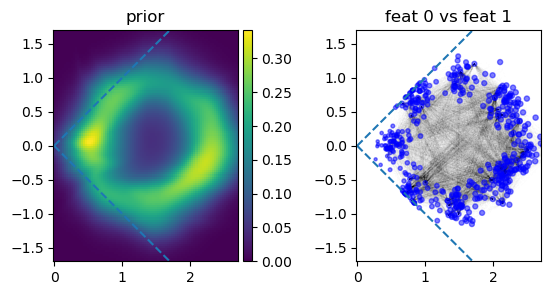
\includegraphics[width=\textwidth]{images/synthetic_2d/circle/pieclam_circ_reconstruct_edges.png}
    %\end{minipage}
    
    %\caption{Left to right: .}
    %\label{fig: pieclam reconstructions}
%\end{figure}

%\endgroup



\subsection{Reconstructing Synthetic SBMs}
\label{sec:reconstruction_sbm}
%\ron{replace with half diagonal sbm comparing the original sbm and approximation of ieclam to bigclam, in the appendix we also show results for pieclam and pclam}
In Figure \ref{fig:sbm_halfdiag} we consider a synthetic SBM with intercommunity connection probability of $0$ and intracommunity connection probability of $0.5$. We sample a simple graph with $N=210$ nodes from the SBM, and fit PClam and PieClam to is. %, and estimate the log cut distance\footnote{We estimate the cut distance underlying the log cut distance using the method from \cite{Alon_cut_estimation2004}.} between the Clam model and the SBM. 
The SBM is off diagonal, so it cannot be well approximated by the PClam model, while the PieClam model approximates it well qualitatively. % (as can be seen by the leftmost and center adjacency matrices in Figure \ref{fig:sbm_halfdiag}).
 %Figure~** illustrates that Clam and PClam models are unable to approximate SBMs which are not diagonally dominant, while IeClam and PieClam can. 
  Additional details are given in Appendix \ref{Extended Details on Experiments}.


\begin{figure}[H] 
\begin{minipage}{0.3\columnwidth} 
\includegraphics[width=\textwidth]{images/sbm_reconstruction/halfdiag.png} \end{minipage}\hfill 
\begin{minipage}{0.3\columnwidth} 
\includegraphics[width=\textwidth]{images/sbm_reconstruction/halfdiag_pieclam/adj.png} \end{minipage} \hfill 
\begin{minipage}{0.3\columnwidth} 
\includegraphics[width=\textwidth]{images/sbm_reconstruction/halfdiag_pclam/adj.png} \end{minipage} 
\caption{Left to right: Original SBM with 3 classes and 9 blocks; Adjacency matrix of the fitted PieClam graph, with two inclusive and two exclusive communities; Adjacency matrix of the fitted PClam graph, with four communities.} 
\label{fig:sbm_halfdiag} 
\end{figure}


% \begin{figure}[!t]
%     \begin{minipage}{0.29\columnwidth}
%         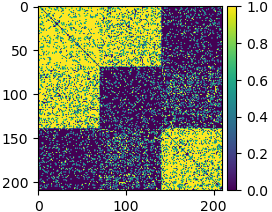
\includegraphics[width=\textwidth]{images/e.png}
        
%     \end{minipage}\hfill
%     \begin{minipage}{0.29\columnwidth}
%         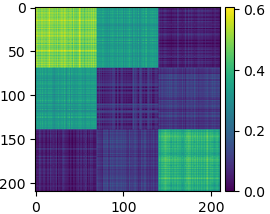
\includegraphics[width=\textwidth]{images/d.png}
        
%     % \end{minipage}\hfill
%     % \begin{minipage}{0.2\columnwidth}
%     %     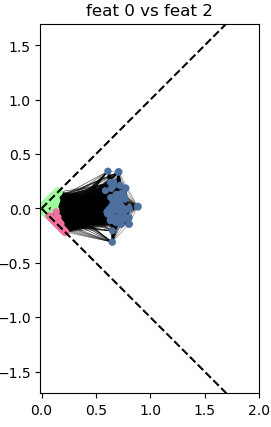
\includegraphics[width=\textwidth]{images/j.png}
        
%     % \end{minipage}
%     % \begin{minipage}{0.2\columnwidth}
%     %     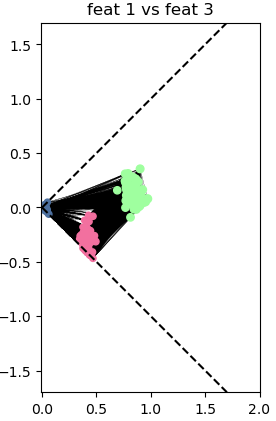
\includegraphics[width=\textwidth]{images/k.png}
        
%     \end{minipage}
%     \caption{Left to right:  Adjacency matrix sampled from SBM with three classes and 9 blocks.  Adjacency matrix of the fitted PieClam graph, with two inclusive and two exclusive communities.  Affiliation features of the PieClam matrix in $\mathcal{T}$ projected to $(t^1,s^1)$ and $(t^2,s^2)$.}
%     \label{fig:sbm_halfdiag}
% \end{figure}

% \begin{figure}[!t]
%     \begin{minipage}{0.3\columnwidth}
%         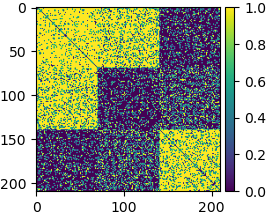
\includegraphics[width=\textwidth]{images/i.png}
        
%     \end{minipage}\hfill
%     \begin{minipage}{0.3\columnwidth}
%         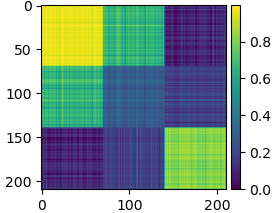
\includegraphics[width=\textwidth]{images/h.png}
        
%     \end{minipage}\hfill
%     \begin{minipage}{0.3\columnwidth}
%         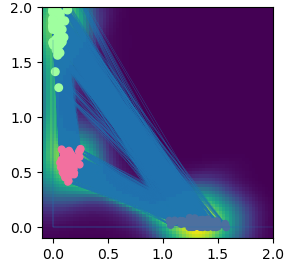
\includegraphics[width=\textwidth]{images/f.png}
        
%     \end{minipage}
%     \caption{Left to right: Adjacency matrix sampled from SBM. Fitted  PClam adjacency matrix based on two inclusive communities.  Affiliations features of the PCLam matrix.}
%     \label{fig:sbm_pclam}
% \end{figure}

\subsection{Anomaly Detection}
\label{sec:anomaly_detection}

In unsupervised node anomaly detection, one is given a graph with node features, where some of the nodes are unknown anomalies. The goal is to detect these anomalous nodes, without supervising on any example of normal or anomalous nodes,  using  only the structure of the graph and the node features.  
%

We  fit a Clam model to the graph and flag nodes as anomalous if they satisfy the following different criteria.
\begin{itemize}
    \item 
    \textbf{(S)} \textbf{Star probability:} Given any Clam model, a node $n$ is called anomalous if $\prod_{m\in\mathcal{N}(n)}P(n\sim m| \mathbf{F})<\delta$. 
    \item 
    \textbf{(P)} \textbf{Prior probability:} Given any Clam model with prior, a node $n$ is called anomalous if $p(\mathbf{f}_n)<\delta$. 
    \item 
     \textbf{(PS)} \textbf{Prior star probability:} Given any Clam model with prior, a node $n$ is called anomalous if $p(\mathbf{f}_n)\prod_{m\in\mathcal{N}(n)}P(n\sim m| \mathbf{F})<\delta$. 
\end{itemize}
 We reduce the dimension of the node features of the input graphs to $100$ using truncated SVD, unless the dimension of the features is smaller than $100$ in which case we only normalize them to have zero mean and standard deviation one.   We use an affiliation space embedding dimension of 30 for $\mathbf{F}$ for PieClam and IeClam, and $24$ for BigClam.
Every Clam method starts with a random embedding $\mathbf{F}$.  Clam models with prior are trained with the following steps. 
 ($\mathbf{F}$-$t$): given a fixed prior $p$, optimize only $\mathbf{F}$ for $t$ steps. ($p$-$t$): given a fixed embedding $\mathbf{F}$, optimize only $p$ for $t$ steps. For regularization, when training, in each iteration of $p$ we add Gaussian noise with STD 0.05 to the affiliation features before plugging them into the prior.  We train PieClam with the scheme $\mathbf{F}$-500 $\rightarrow$ $p$-1300 $\rightarrow$ $\mathbf{F}$-500 $\rightarrow$ $p$-1300 $\rightarrow$ $\mathbf{F}$-500 $\rightarrow$ $p$-1300 with learning rate of $2e^{-6}$ on $\mathbf{F}$  and $1e^{-6}$ on $p$.
 In every alternation between two $(p-t)$ and $(\mathbf{F}-t)$ schemes, both learning rates are decreased by a factor of $2$.
For the models which only optimize $\mathbf{F}$ (IeClam and BigClam)  we use the following configurations. We train IeClam with 2500 iterations with learning rate 1e-6. We train BigClam with 2200 iterations with learning rate 1e-6.
More details on hyper-parameters are given in Appendix \ref{sec: additional experiments anomaly}, and in our GitHub repository.


In Table~\ref{Table1} we compare the performance of Clam methods to DOMINANT \cite{ding2019dominant}, AnomalyDAE \cite{fan2020anomalydae}, OCGNN \cite{wang2021ocgnn}, AEGIS \cite{ding2021aegis}, GAAN \cite{chen2020gaan} and TAM \cite{qiao2024tam} on the datasets Reddit, Elliptic \cite{elliptic} \cite{elliptic2}, and Photo \cite{photo}. The hyper-parameters of the competing methods are taken as the recommended values from the respective papers. The results are taken from Table 1 in \cite{qiao2024ggad}.
We observe that our methods are the first and second place on all datasets. Moreover, (PS)- PieClam beats the competing  methods in all  three datasets. %\dan{the results have changed so can maybe say somethign stronger. Also S-PieClam should also be mentioned if we leave this sentence}

ִ
%elliptic
%accuracies_anomaly['vanilla_star'][-1]= 0.43547641111559626
%        accuracies_anomaly['prior'][-1]= 0.6092925420504949
%        accuracies_anomaly['prior_star'][-1]= 0.550598487402

%reddit
%accuracies_anomaly['vanilla_star'][-1]= %0.6104237623089773
 %       accuracies_anomaly['prior'][-1]= 0.5671389289452801
 %       accuracies_anomaly['prior_star'][-1]= 0.6124879959487293

%photo
%accuracies_anomaly['vanilla_star'][-1]= 0.5564428423968186
%        accuracies_anomaly['prior'][-1]= 0.42471794085192105
%        accuracies_anomaly['prior_star'][-1]= 0.5065087026473599

        

\begin{table}[t]
\footnotesize
\centering
\begin{tabular}{|c|c|c|c|}
    \hline
  Method  & Reddit& Elliptic& Photo\\
    \hline

%  (S)- IeClam& \underline{64.1}& 0.2&\textbf{0.592}\\
%  (S) - PieClam & \textbf{0.640} & 0.435 & \underline{0.590} \\
% (P) - PieClam & 0.468 & \textbf{0.632} & 0.457 \\
% (PS) - PieClam & \textbf{0.640} & \underline{0.538} & \underline{0.590} \\
%  (S) - BigClam & 0.637& 0.434&0.581\\
%  \hline
%  DOMINANT  & 0.511& 0.296&0.514\\
%  AnomalyDAE &0.509& *0.496&0.507\\
%  OCGNN  &0.525 & 0.258&0.531\\
%  AEGIS &0.535 & 0.455&0.552\\
%  GAAN &0.522 &0.259 &0.430\\
%  TAM &0.606 & 0.404 & 0.568\\
(S)- IeClam & \textbf{64.1} & 43.6 & 57.7 \\
(S) - PieClam & *64.0 & 43.5 & \underline{59.0} \\
(P) - PieClam & 46.8 & \textbf{63.2} & 45.7 \\
(PS) - PieClam & \underline{64.0} & \underline{53.8} & \textbf{59.0} \\
(S) - BigClam & 63.7 & 43.4 & *58.1 \\
\hline
DOMINANT & 51.1 & 29.6 & 51.4 \\
AnomalyDAE & 50.9 & *49.6 & 50.7 \\
OCGNN & 52.5 & 25.8 & 53.1 \\
AEGIS & 53.5 & 45.5 & 55.2 \\
GAAN & 52.2 & 25.9 & 43.0 \\
TAM & 60.6 & 40.4 & 56.8 \\
 \hline
\end{tabular}
\caption{Comparison of Clam anomaly detectors with competing methods. % to DOMINANT \cite{ding2019dominant}, AnomalyDAE \cite{fan2020anomalydae}, OCGNN \cite{wang2021ocgnn}, AEGIS \cite{ding2021aegis}, GAAN \cite{chen2020gaan} and TAM \cite{qiao2024tam}. 
 First place in \textbf{boldface}, second with \underline{underline}, third with *star. %We observe that our methods are first and second place on all datasets. Moreover, S- IeClam, PS-PieClam and S BigClam each beats the competing methods in two out of the three datasets. 
 The accuracy metric is areas under curve (AUC).}
\label{Table1}
\end{table}

%\begingroup
%\color{blue}
\subsection{Link Prediction}
In supervised link prediction, one is given a graph where for  some of the dyads it is unknown if they are edges or not. The goal is to predict the connectivity of the omitted dyads. Given a Clam model fitted to the known data, we predict the probability of an edge using the conditional probability given in (\ref{eq:LorFeature}). In our experiments, the prior and features are not directly used for prediction, but they are used to train the Clam model if it has a prior. %and we do not use the features. Hence, our link prediction method only uses the graph structure. 
In Appendix \ref{sec: link prediction experiment} we show that the log likelihood, restricted to the known dyads, can be efficiently computed by
\[\footnotesize
\begin{split}
2\hat{l}(\mathbf{F}, E, \check{\mathcal{E})}=&2\underset{n\in [N]}{\sum} \log(p(\mathbf{f}_n)) 
+ \hspace{-2.0mm}\underset{(n,m)\in E\setminus\check{E}}{\sum} \log(1-e^{-\mathbf{f}_n^\top \mathbf{L} \mathbf{f}_m}) \\
&- \underset{n\in [N]}{\sum} \mathbf{f}_n^\top \underset{m\in [N]}{\sum} \mathbf{L} \mathbf{f}_m
+\underset{(n,m)\in E \dot{\cup} \check{\overline{E}}\dot{\cup}D}{\sum} \mathbf{f}_n^\top \mathbf{L} \mathbf{f}_m
\end{split}
\]
%\[%\begin{equation}
%\footnotesize
%\begin{split}
%& \underset{(n,m)\in E\setminus\check{E}}{\sum} \log(e^{\mathbf{f}_n^\top \mathbf{L} \mathbf{f}_m}-1) - \underset{(n,m)\in \mathcal{E}}{\sum} \mathbf{f}_n^\top \mathbf{L} \mathbf{f}_m + \sum_{n \in [N]} \mathbf{f}_n^\top \mathbf{L} \mathbf{f}_n\\ 
%&+ \underset{(n,m) \in \check{\mathcal{E}}}{\sum}\mathbf{f}_n^\top \mathbf{L} \mathbf{f}_m.\,
%\end{split}
%\label{def: link loss}
%\end{equation}
%\]
 where $E$ is the set of edges,  $\check{E}$ is the set of omitted edges,  $\check{\overline{E}}$ is the set of omitted non-edges,  $\check{\mathcal{E}}= \check{E}\dot{\cup}\check{\overline{E}}$ is the set of omitted dyads, and $D=\{(n,n)| n\in [N]\}$. %\dan{danny: Note that this expression is in fact the sum of the original PieClam loss on the retained edge set and an L-product on the omitted edges (should make the long expression easier to understand)} 
  This computation is as efficient as message passing when the number of omitted non-edges is of the same order as $E$. 
After assigning probabilities to all of the omitted dyads, we calculate the AUC score of the classification.
We use the experimental setting presented in \cite{zhou2022disenlink}.  



For each dataset, we generate 10 random splits into a test set  containing $10\%$ of the edges, along with 5 randomly sampled non-edges for every omitted edge, and the rest is the training set. For each split and each configuration of the hyperparameters, we generate three random validation sets consisting of $5\%$ of the edges from the training set and 5  non-edges per omitted edge also from the training set, leaving the rest of the original training set for training.  We perform hyperparameter optimization as follows: Each hyperparameter configuration is trained against each of its respective 30 training sets, and its accuracy is evaluated over the corresponding 30 validation sets and averaged to obtain one mean validation accuracy per configuration. We then choose the configuration with maximal mean validation accuracy. The model with these optimal hyperparameters  is then trained on each of the original 10 training sets and tested on each of the corresponding test sets, 10 times for each split. We report the mean accuracy across the 100 trained models on the 10 test sets, along with the standard deviation of the mean. 

\dan{
For each dataset we generate 10 random splits into a test set containing 10\% of the edges, along with 5 randomly sampled non-edges for every omitted edge, and the rest is the training set. For each split and each configuration of the
hyperparameters, we generate three random validation sets
consisting of 5% of the edges from the training set and 5 non-
edges per omitted edge also from the training set, leaving
the rest of the original training set for training. 
We fix the first function in the optimization to be $\mathbf{F} - t$ and the prior noise STD to be 0.1. We also set the l${_1}$ regularization to $1$ and for the IE models we set the $\mathbf{s}$ community regularization to $0.1$. The possible configurations are taken from the following parameter ranges: 
}


We run our experiments on the datasets Squirrel and Texas \cite{pei2020texasquirrel}, Photo \cite{shchur2018photo} and Facebook100's Johns Hopkins \cite{lim2021hopkins}, and compare PieClam to the baselines AA \cite{adamic2003friends}, VGAE \cite{kipf2016variational}, GAT \cite{GAT}, LINKX \cite{lim2021linkx} and Disenlink \cite{zhou2022disenlink}. The results are presented in Table \ref{table: link table0} (and with error bars in Table \ref{table: link table}),  %\dan{danny: an interesting result omitted from the table is IeClam on texas which gives an auc score of $80.0 \pm 2.0$ and takes only 10 seconds to train (second place is disenlink with $81.0 \pm 4.0$ so it's the same as Ieclam basically...)} 
 and the baseline results are taken from Table 2 in \cite{zhou2022disenlink}. An in depth explanation on the experimental setup and a table with confidence intervals is given in Appendix \ref{sec: link prediction experiment}.
 \begin{table}[t]
 \footnotesize
    \centering
    \begin{tabular}{|c|c|c|c|c|}
        \hline
        Method  & Squirrel        & Photo           & Texas        & JH55 \\
        \hline
        PieClam & \textbf{98.7} & \textbf{98.4}     &   \textbf{85.0}           & 95.5*     \\
        \hline
        BigClam & \underline{98.5}& 97.4 *  & 78.2 *& 94.9  \\
        VGAE    &   98.2   &94.9   & 68.6  & 92.8  \\
        GAT     &   98.0    &97.3   & 68.5  &   94.3 \\
        LINKX   &   98.1    &97.0   & 75.8  &   93.4  \\
        AA      &   97.1  &97.4   & 53.1  &  \underline{96.1}  \\
        DisenLink & 98.3* & \underline{97.9} & \underline{81.0} &   \textbf{97.5} \\
        \hline
    \end{tabular}
    \caption{Comparison of Clam link predictors with competing models. First place in \textbf{boldface}, second with \underline{underline}, third with *star}
    \label{table: link table0}
\end{table}


We conducted additional link prediction experiments on the \textbf{OGB-DDI} dataset. In this dataset, nodes represent different drugs, and an edge between two nodes indicates that a different effect occurs when the drugs are taken together versus separately. Our model achieves state-of-the-art performance on this benchmark in terms of the \textbf{Hits@20} metric (using OGB's official evaluator). 
A comparison between our model (\textbf{IeClam}) and selected baselines on the dataset's test set is presented in Table \ref{table:ddi-results}. Benchmark results are taken from~\cite{zhang2022unsupervised,li2023evaluating,tan2022mgae}. 
\begin{table}[t]
 \footnotesize
    \centering
    \begin{tabular}{|l|c|c|}
        \hline
        \textbf{Model} & \textbf{Hits@20 (Test)} & \textbf{AUC (Test)} \\
        \hline
        \textbf{IeClam}   & \textbf{88.10 $\pm$ 1.70} & 99.84 $\pm$ 0.01 \\
        \cline{1-3}
        NCN              & 76.52 $\pm$ 10.47 & \textbf{99.97 $\pm$ 0.00} \\
        GraphSAGE        & 49.84 $\pm$ 15.56 & 99.96 $\pm$ 0.00 \\
        GCN              & 49.90 $\pm$ 7.23  & 99.86 $\pm$ 0.03 \\
        BUDDY            & 29.60 $\pm$ 4.75  & 99.81 $\pm$ 0.02 \\
        Node2Vec         & 34.69 $\pm$ 2.90  & 99.78 $\pm$ 0.04 \\
        \hline
    \end{tabular}
    \caption{Performance on the OGB-DDI dataset. First place is in \textbf{boldface}.}
    \label{table:ddi-results}
\end{table}

%\endgroup


%We note that all of the competing models require the use of node attributes to recognize anomalies. One advantage of our models is that we often do not require the graph to have node attribute to achieve competitive results (in \ron{name the graphs in which we do not need features to be good}). 

\section{Conclusion}

We introduced PieClam, a new probabilistic graph generative model. PieClam models graphs via embedding the nodes into an inclusive and exclusive communities space, learning a prior distribution in this space, and decoding pairs of points in this space to edge probabilities, such that points are more likely to be connected the more inclusive communities and the less exclusive communities they share. We showed that PieClam is a universal autoencoder, able to approximate any graph, where the budget of parameters per node (the number of communities) can be predefined, irrespective of any property of a specific graph, not even the number of nodes. Our experiments show that PieClam achieves competitive results when used in graph anomaly detection.

One limitation of PieClam is that, for attributed graphs, it only models the node features through the prior in the community affiliation space, but not via the conditional probabilities of the edges (given the community affiliations). Future work will deal with extending PieClam to also include the node (or edge) features in the edge conditional probabilities. 
Another limitation is in the analysis. While our methods performs well for sparse graphs, our analysis involving the log cut distance is mainly appropriate for dense graphs. Indeed, the term $1/N^2$ in (\ref{eq:KL2}) leads all sparse graphs  with $|E|\ll N^2$  to be trivially close to each other.  Future work will extend our log cut similarity measure  to sparse graphs.  This can be done, e.g., similarly to the sparse theory in \cite{Levie_intersecting_reg_24}, or using stretched graphons \cite{JMLR:v18:16-421}, $L^p$ graphons \cite{Borgs2014AnT}, graphings \cite{cut-homo3} or graphops \cite{Backhausz2018ActionCO}.

%\clearpage

\section*{Impact Statement}
This paper presents work whose goal is to advance the field of 
Machine Learning. There are many potential societal consequences 
of our work, none which we feel must be specifically highlighted here.

\section*{Acknowledgments}

This research was supported by a grant from the United States-Israel Binational Science Foundation (BSF), Jerusalem, Israel, and the United States National Science Foundation (NSF), (NSF-BSF, grant No. 2024660), and by the Israel Science Foundation (ISF grant No. 1937/23).

\bibliography{bibiliography}
\bibliographystyle{icml2025}
\[\]



\clearpage


%\subsection{Ablation Study}
%\textcolor{cyan}{should i refer only to the anomaly detection or also to the shape experiments?}
%\paragraph{Large Learning Rate for Feature Optimization}
%If the learning rate for the feature optimization is too large...

%\paragraph{Relationship Between Prior and Feature Optimization Parameters}
%Write what happens when you change the archtiecture.

%Without feature noise?

%Different nbumber of iterations?

%Optimizing the prior together with the Clam features?



%%%%%%%%%%%%%%%%%%%%%%%%%%%%%%%%%%%%%%%%%%%%%%%%%%%%%%%%%%%%%%%%%%%%%%%%%%%%%%%
%%%%%%%%%%%%%%%%%%%%%%%%%%%%%%%%%%%%%%%%%%%%%%%%%%%%%%%%%%%%%%%%%%%%%%%%%%%%%%%
% APPENDIX
%%%%%%%%%%%%%%%%%%%%%%%%%%%%%%%%%%%%%%%%%%%%%%%%%%%%%%%%%%%%%%%%%%%%%%%%%%%%%%%
%%%%%%%%%%%%%%%%%%%%%%%%%%%%%%%%%%%%%%%%%%%%%%%%%%%%%%%%%%%%%%%%%%%%%%%%%%%%%%%
\newpage
\appendix
\onecolumn

\appendix

\begin{center}
{\huge \textbf{Supplementary Material}}


\end{center}

\section{Proofs}

\subsection{Proof That BigClam Is Not Universal}
\label{Proof That BigClam Is Not Universal}
In this subsection we Prove Claim \ref{claim:Clam_bi}. 
Consider the bipartite graph $\mathbf{B}$ with $N$ nodes at each part, and probability $1-e^{-a^2}$ for an edge between the two parts, and $0$ within each part. Consider (\ref{eq:KL3}) as the definition of the log cut distance. Let $\mathbf{P}$ be a decoded BigClam graph from the affiliation features $\mathbf{F}$.

Denote by $\tilde{\mathbf{P}}$ the matrix with entries 
\[\tilde{p}_{n,m}=-\log(1-p_{n,m})=\mathbf{f}_n^\top\mathbf{f}_m,\] 
and by $\tilde{\mathbf{B}}$ the matrix  with entries $\tilde{b}_{n,m}=-\log(1-b_{n,m})$.
We show that there is no way to make $\| \tilde{\mathbf{P}}-\tilde{\mathbf{Q}}\|_{\square}$ small.

\begin{claim}
    Under the above construction, 
    \[D^0_{\square}(\mathbf{P} || \mathbf{B}) \geq \frac{a^2}{16}.\]
    As a result, BigClam is not a universal autoencoder.
\end{claim}


\begin{proof}
    
Note that $\tilde{b}_{n,m}=a^2$ if $n,m$ are in opposite parts, and $\tilde{b}_{n,m}=0$ if $n,m$ are on the same side.
We index the nodes such that $[N]$ is the first side of the graph, and $[N]+N$ is the second side. For $n\in[N]$ we denote $\mathbf{q}_n=\mathbf{f}_n$ and  $\mathbf{y}_n=\mathbf{f}_{n+N}$.
Next, we use the identity 
\[D^0_{\square}(\mathbf{P} || \mathbf{Q}) = \| \tilde{P}-\tilde{B}\|_{\square },\]
and bound the right-hand-side from below.

First, by the definition of cut norm, for every $\mathcal{U},\mathcal{V}\subset[2N]$,
\[\| \tilde{P}-\tilde{B}\|_{\square} \geq \Big|\frac{1}{4N^2}\sum_{n\in \mathcal{U}}\sum_{m\in \mathcal{V}} (\tilde{p}_{n,m} - \tilde{b}_{n,m})\Big|.\]
Hence, for $\mathcal{U}_1=\mathcal{V}_1=[N]$, $\mathcal{U}_2=\mathcal{V}_2=[N]+1$, $\mathcal{U}_3=[N],\mathcal{V}_3=[N]+N$, and $\mathcal{U}_4=[N]+N,\mathcal{V}_4=[N]$, we have
\[\| \tilde{P}-\tilde{B}\|_{\square} \geq \frac{1}{16N^2}\sum_{j=1}^4 \Big|\sum_{n\in \mathcal{U}_j}\sum_{n\in \mathcal{V}_j} (\tilde{p}_{n,m} - \tilde{b}_{n,m})\Big| \]
\begin{equation}
    \label{eq:ClamNpUni0}
= \frac{1}{16N^2}\sum_{n=1}^N\sum_{m=1}^{N} \mathbf{q}_n^\top \mathbf{q}_m  + \frac{1}{16N^2}\sum_{n=1}^N\sum_{m=1}^{N} \mathbf{y}_n^\top \mathbf{y}_m 
    +\frac{1}{8N^2}\sum_{n=1}^N\sum_{m=1}^{N} ( a^2 -\mathbf{q}_n^\top \mathbf{y}_m).
\end{equation}


Denote 
\[\mathbf{q}=\frac{1}{N}\sum_{n=1}^N \mathbf{q}_n, \quad \mathbf{y}=\frac{1}{N}\sum_{n=1}^N \mathbf{y}_n.\]
With these notations, (\ref{eq:ClamNpUni0}) can be written as
{\color{orange}
\[\| \tilde{P}-\tilde{B}\|_{\square} \geq \]
\[\frac{1}{16}\mathbf{q}^\top \mathbf{q}  + \frac{1}{16}\mathbf{y}^\top \mathbf{y} +\frac{1}{8}( a^2 -\mathbf{q}^\top \mathbf{y})\]
\[=\frac{1}{16}\Big(a^2 + (\mathbf{q}^\top-\mathbf{y}^\top)(\mathbf{q}-\mathbf{y})\Big) \geq \frac{a^2}{16}.\]
}
\dan{
\[\| \tilde{P}-\tilde{B}\|_{\square} \geq \frac{1}{16}\mathbf{q}^\top \mathbf{q}  + \frac{1}{16}\mathbf{y}^\top \mathbf{y} +\frac{1}{8}( a^2 -\mathbf{q}^\top \mathbf{y}) = \frac{1}{16}\Big(a^2 + (\mathbf{q}^\top-\mathbf{y}^\top)(\mathbf{q}-\mathbf{y})\Big) \geq \frac{a^2}{16}.\]
}
\end{proof}

We note that one can similarly show that BigClam is not universal also with respect to the log cut distance of Definition \ref{def:KL2}.





















\subsection{BigClam With No Self Loops Approximating Bipartite Graphs}
\label{BigClam With No Self Loops Approximating Bipartites}

Consider the above bipartite graph  $\mathbf{B}$ with $N$ nodes at each part, and probability $1-e^{-a^2}$ for an edge between the two parts, and $0$ within each part. 
If we redefine the BigClam decoder to have no self-loops, namely, $\mathbf{P}$ has entries 
$p_{n,m}=P(n\sim m|\mathbf{f}_n, \mathbf{f}_m)$ for $n\neq m$, and $p_{n,m}=0$ for $n=m$, then one can obtain a bipartite $\mathbf{P}$ with $C=N^2$ communities as follows. 

In the following analysis, an addition or multiplication of a set by a scalar is defined to be the addition or multiplication of every element in the set by this scalar.
Encode each node $n\in[N]$ in part 1 to $\mathbf{f}_n$ with
$f_n^c=a$ for {\color{orange}$c\in [N]+n(N-1)$} \dan{$c\in [N] + N(n-1)$} and $f_n^c=0$ otherwise. Encode every node $n\in [N]+N$ from side 2 to $\mathbf{f}_n$ with
$f_n^c=a$ for $c\in N([N]-1)+n$ and $f_n^c=0$ otherwise. It is easy to see that the corresponding $\mathbf{P}$ is bipartite with edge probability between the parts being $1-e^{-a^2}$.






\subsection{Proof of the Universality of PieClam}
\label{Proof of the Universality of PieClam}

The proof is based on a version of the weak regularity lemma for intersecting communities. While the standard weak regularity lemma \cite{weakReg,Szemeredi_analyst} partitions the graph into disjoint communities, it is well known that allowing the communities to overlap allows using much less communities, which improves the asymptotics of the approximation. The regularity lemma was used in the context of graph machine learning in \cite{Levie_reg_23,Levie_intersecting_reg_24}. To formalize the relevant version of the weak regularity theorem for our analysis, we first need to cite a definition from \cite{Levie_intersecting_reg_24}.

\begin{definition}
    A (hard) intersecting community graph (ICG) with $N$ nodes and  $K$ communities is a matrix $\mathbf{C}\in\mathbb{R}^{N\times N}$ of the following form. There exist $K$ column vectors $\mathbf{Q}=\big(\mathbf{q}_k\in\{0,1\}^N\big))_{k=1}^K\in \{0,1\}^{N\times K}$ and $k$ coefficients $\mathbf{r}=(r_k\in\mathbb{R})_{k=1}^K\in\mathbb{R}^K$ such that
    \[\mathbf{C}= \mathbf{Q}{\rm diag}(\mathbf{r})\mathbf{Q}^{\top }.\]
\end{definition}

%\ron{Prove in the supplamentry material the regularity lemma for non-negative $A$ approximated by non-negatieve $C$. For this, we can replace the 0 values of $A$ by small $\delta>0$. Then, cancel a DC part (full community) to $C$... Or just go over the proof...}

%\ron{Follow the standard proof, and demand positivity of the approximant each time. For that follow the proof of the lemma in Hilbert space in the special case of functions. Seems like the Hilbert regularity lemma should work with this restriction. Indeed, I am looking for a step where there is not a big improvement.}

%\ron{However, the thing I am allowed to take inner product against in this lemma would also be something that together with prevous approximation would be positive. This is fine! Since I only want to take inner product against tensor indicators with positive coefficient!!! So it works!}

The following is a special case of the weak regularity lemma from \cite{Levie_intersecting_reg_24}, up to the small modification to the adjacency matrix, allowing it to have values in $[0,R]$ instead of $[0,1]$. %, it is well known as a step in the proof of the weak regularity lemma, see, .e.g  [Frieze, Fast. , Lovasz. Analyst]. For completness, we prove it in Appendix ***.

\begin{theorem}
\label{thm:reg_sprase}
   % Let $1\leq p\leq2$. % and $D\in\sN$.
     Let $\mathbf{A}\in[0,R]^{N\times N}$ be an adjacency matrix of a graph with $N$ nodes. Let $\epsilon>0$. Denote $K=\frac{9R^2}{4\epsilon^2}$. Then, there exists a hard ICG $\mathbf{C}$ with $K$ communities such that 
    \begin{equation}
        \label{eq:reg_sparse}
    \|\mathbf{A}-\mathbf{C}\|_{\square} \leq \epsilon.
    \end{equation}
\end{theorem}

\begin{proof}[Proof of Theorem \ref{thm:IEUniversality}]
 Let $\epsilon>0$. Let $\mathbf{A}\in[0,1]^{N\times N}$ be an adjacency matrix. Let $0<d\leq 1$.

Consider the matrix  $\tilde{\mathbf{A}}$ with entries
\[\tilde{a}_{n,m}=-\log(1-(1-d)a_{n,m}).\]
In the following construction, we build IeClam affiliation features $\mathbf{F}$ and we want
\[1-\exp(-\mathbf{f}_n^{\top}\mathbf{L}\mathbf{f}_m)\approx (1-d)a_{n,m}.\]
%So the regularity lemma should be against the matrix $\mathbf{X}$ with entries
%\[x_{u,v}=-\log(1-(1-d)a_{u,v}).\]
Note that $-\log(1-(1-d)a_{n,m})$ is increasing in $(1-d)a_{n,m}$. For $(1-d)a_{n,m}=0$ the value of this function is 0, and for $(1-d)a_{n,m}=1-d$ it is $R=-\log(d)$. Choose $d=\epsilon/2$. For this specific choice of $d$, if we replace $d$ by $\epsilon/2$ in the definition of $D_{\square}$ and omit the infimum, we get an upper bound of $D_{\square}(\mathbf{P},\mathbf{A})$.
 

%We now use the overlapping weak regularity lemma.


Using the overlaping weak regularity lemma, we approximate $\tilde{\mathbf{A}}$ by an ICG with 
\[K=\frac{-9\log(\epsilon/2)^2}{\epsilon^2}\]
communities,
\[\mathbf{C}= \mathbf{Q}{\rm diag}(\mathbf{r})\mathbf{Q}^{\top },\]
such that
\[\|\tilde{\mathbf{A}}-\mathbf{C}\|_{\square} \leq \epsilon/2.\]

Let $\mathbf{r}_+={\rm ReLU}(\mathbf{r})$ and $\mathbf{r}_-={\rm ReLU}(-\mathbf{r})$. Denote
\[\mathbf{C}_+=\mathbf{Q}{\rm diag}(\sqrt{\mathbf{r}_+})\]
and
\[\mathbf{C}_-=\mathbf{Q}{\rm diag}(\sqrt{\mathbf{r}_-}).\]
Denote the rows of $\mathbf{C}_+$ by $\mathbf{t}_n$ and the rows of $\mathbf{C}_-$  by $\mathbf{s}_n$, for $n=1,\ldots,N$. For each $n\in[N]$ we concatenate $(\mathbf{t}_n,\mathbf{s}_n)$ to define the affiliation feature $\mathbf{f}_n$, with the first $K$ coordinates being the inclusive communities, and the last $K$ coordinates being the exclusive communities. Denote the corresponding IeClam matrix by $\mathbf{P}$.

It is easy to see that $\mathbf{f}_n^\top\mathbf{L}\mathbf{f}_m$ is the $(n,m)$ entry of $\mathbf{Q}{\rm diag}(\mathbf{r})\mathbf{Q}^{\top }$. 
%Hence, since $\mathbf{C}$ is non-negative, the set $\{\mathbf{f}_n\}_{n\in[N]}$ belongs to some cone $\mathbf{C}$.
This also proves that
{\color{orange}
\[\|-\log(1-(1-\epsilon)\mathbf{A})+\log(1-\mathbf{P})\|_{\square}\]
\[=\|\tilde{\mathbf{A}}-\mathbf{C}\|_{\square} \leq \epsilon/2.\]
}
\dan{
\[\|-\log(1-(1-\epsilon)\mathbf{A})+\log(1-\mathbf{P})\|_{\square} = \|\tilde{\mathbf{A}}-\mathbf{C}\|_{\square} \leq \epsilon/2.\]
}
%The claim now follows by adding $\epsilon$ to the above formula, and then replacing $\epsilon$ by $\epsilon/2$.
%
We can now summarize
{\color{orange}
\[D_{\square}(\mathbf{P}||\mathbf{A}) \leq \]
\[\epsilon/2+\frac{1}{N^2}\sup_{\mathcal{U},\mathcal{V}\subset[N]}\Big|\log\Big(\prod_{n\in \mathcal{U}}\prod_{m\in \mathcal{V}}
\frac{1-p_{n,m}}{1-(1-\epsilon/2)a_{n,m}}\Big)\Big|\]
\[ =
\epsilon/2+\frac{1}{N^2}\sup_{\mathcal{U},\mathcal{V}\subset[N]}\Big|\sum_{n\in \mathcal{U}}\sum_{m\in \mathcal{V}}\Big(-\log\big(1-(1-\epsilon)a_{n,m}\big) \]
\[\quad \quad \quad \quad\quad \quad \quad \quad + \log\big(1-p_{n,m})\big)\Big)\Big|\]
\[=\epsilon/2 + \| \tilde{\mathbf{P}}-\mathbf{C} \|_{\square} = \epsilon. \]
}
\dan{
\[D_{\square}(\mathbf{P}||\mathbf{A}) \leq \epsilon/2+\frac{1}{N^2}\sup_{\mathcal{U},\mathcal{V}\subset[N]}\Big|\log\Big(\prod_{n\in \mathcal{U}}\prod_{m\in \mathcal{V}}
\frac{1-p_{n,m}}{1-(1-\epsilon/2)a_{n,m}}\Big)\Big|\]
\[ =
\epsilon/2+\frac{1}{N^2}\sup_{\mathcal{U},\mathcal{V}\subset[N]}\Big|\sum_{n\in \mathcal{U}}\sum_{m\in \mathcal{V}}\Big(-\log\big(1-(1-\epsilon)a_{n,m}\big) + \log\big(1-p_{n,m})\big)\Big)\Big|\]
\[=\epsilon/2 + \| \tilde{\mathbf{P}}-\mathbf{C} \|_{\square} = \epsilon. \]
}
\end{proof}


\subsection{Proof of the Universality of IeClam in the Pairwise Cone of Non-negativity}
\label{Proof of the Universality of IeClam in a Cone of Non-negativity}

For this result, we use the standard weak regularity lemma for non-intersecting classes.  It is based on the weak regularity lemma from \cite{weakReg,Szemeredi_analyst}, see also Lemma 9.3 and Corollary 9.13 from \cite{cut-homo3}.

\begin{definition}
    A \emph{block matrix} $\mathbf{B}$ with $K$ classes is a symmetric matrix $\mathbf{B}\in[0,\infty)^{N\times N}$ for which there exists a partition of $[N]$ into $K$ disjoint sets, called \emph{classes}, $\mathcal{C}_1,\ldots,\mathcal{C}_K$ (with $\cup\mathcal{C}_j=[N]$), such that for every pair of classes $i,j\in[K]$, there is a constant $c_{i,j}\geq 0$ such that  $b_{n,m}=c_{i,j}$ for any two nodes $n\in\mathcal{C}_i$ and $m\in\mathcal{C}_j$.
\end{definition}

%Since we need our approximating block matrix to be non-negative, we
%Denote the \emph{Frobenius} norm of a matrix $\mathbf{X}\in\mathbb{R}^{N\times N}$ by
%\[\|\mathbf{X}\|_{\rm F} = \sqrt{\sum_{n,m=1}^N x_{n,m}^2}.\]
\begin{theorem}
\label{thm:reg_sprase2}
   % Let $1\leq p\leq2$. % and $D\in\sN$.
     Let $\mathbf{A}\in[0,R]^{N\times N}$ be an adjacency matrix of a graph with $N$ nodes. Let $\epsilon>0$. Denote $K=2^{2\lceil R^2/\epsilon^2\rceil}$.         Then, there exists a block matrix  $\mathbf{B}$ with $K$ (disjoint) classes such that 
    \begin{equation}
        \label{eq:reg_sparse2}
    \|\mathbf{A}-\mathbf{B}\|_{\square} \leq \epsilon.
    \end{equation}
    %and 
    %\[\|\mathbf{A}-\mathbf{B}\|_{\rm F} = \min_{\mathbf{B}'} \|\mathbf{A}-\mathbf{B}'\|_{\rm F},\]
    %where the minimum is over the block matrices $\mathbf{B}'$ with $K$ (disjoint) classes. 
\end{theorem}
%Note that Theorem \cite{Levie_intersecting_reg_24} is for intersecting classes. Our Theorem \ref{thm:reg_sprase2} follows \cite{Levie_intersecting_reg_24}  by two simple modifications.
%First, by scaling $[0,R]$-valued adjacency matrices to be $[0,1]$ valued. Second, by taking deriving $K=2^M$ non-intersecting classes  $\mathcal{C}=\{\mathcal{C}_j\}_{j=1}^K$ from the $M=9R^2/4\epsilon^2$ intersecting classes $\mathcal{Q}=\{\mathcal{Q}_j\}_{j=1}^M$ via
% \[\tilde{\mathcal{C}}=\big\{C\subset [0,1] \ |\ \exists ~n\in[N]: ~C=\cap\{\mathcal{Q}_j\in\mathcal{Q}|n\in \mathcal{Q}_j\}\big\},\]
% and adding to $\tilde{\mathcal{C}}$ as many copies of the empty set to obtain $K=2^M$ disjoint sets $\mathcal{C}.$

%The last part of Theorem \ref{thm:reg_sprase2} is useful for showing that we may take $\mathbf{B}$ to be non-negative. 
%Indeed, since $\mathbf{A}$ is non-negative, replacing any negative block of $\mathbf{B}$ by a block of zeros can only improve the Frobenius approximation. 

We stress that Theorem \ref{thm:reg_sprase2} guarantees non-negative block values of $\mathbf{B}$, while in Theorem \ref{thm:reg_sprase}, in general, the matrix $\mathbf{C}$ may have negative entries.

%Hence, as a corollary of Theorem \ref{thm:reg_sprase2}, under the same assumptions, there exists a non-negative $\mathbf{B}$ that satisfies $\|\mathbf{A}-\mathbf{B}\|_{\square} \leq \epsilon$. 







\begin{proof}[Proof of Theorem \ref{thm:IEUniversality2}]

We start similarly to the proof of Theorem \ref{thm:IEUniversality}. Let $\epsilon>0$. Let $\mathbf{A}\in[0,1]^{N\times N}$ be an adjacency matrix. 
Consider the matrix  $\tilde{\mathbf{A}}\in[0,-\log(\epsilon/2)]$ with entries
\[\tilde{a}_{n,m}=-\log(1-(1-\epsilon/2)a_{n,m}).\]
In the following, we build IeClam affiliation features $\mathbf{F}$  such that
\[1-\exp(-\mathbf{f}_n^{\top}\mathbf{L}\mathbf{f}_m)\approx (1-\epsilon/2)a_{n,m}.\]

By the weak regularity lemma (Theorem \ref{thm:reg_sprase2}), we approximate there is a non-negative block matrix $\mathbf{B}$ with $K=2^{2\lceil -\log(\epsilon/2)^2/\epsilon^2\rceil}$ classes $\mathcal{C}_1,\ldots,\mathcal{C}_K$, such that
\[\|\tilde{\mathbf{A}}-\mathbf{B}\|_{\square} \leq \epsilon.\]

We now take the affiliation space to have $C=K^2$ inclusive communities  and $C=K^2$ exclusive communities.

For each $n\in[N]$, let $k_n$ be the class such that $c\in\mathcal{C}_{n_k}$.  For each pair of classes $i,j\in[K]$, let $c_{i,j}\geq 0$ denote the edge weight between $\mathcal{C}_i$ and $\mathcal{C}_j$.
%Build a feature for every block. $\mathbf{f}_n$ is:

%I have enough dimensions to make each $n$ that belong to the same class to interact as I wish with all of the other classes.

%Let $c_{i,j}$ be the block values. let $k_n$ be the class of node $n$. Then we build the features by:

The feature of each $n\in[N]$ at the inclusive channel $c=(K-1)k_n+k_n$ is $t_n^c=\sqrt{c_{k_n,k_n}}$. It is $t_n^c=\sqrt{c_{k_n,j}/4}$ at inclusive channels $c=(K-1)k_n+j$ and $c=(K-1)j+k_n$, and $s_n^c=-\sqrt{c_{k_n,j}/4}$ at exclusive channels $c=(K-1)k_n+j$ and $c=(K-1)j+k_n$. In all other channels $t^c_n$ and $s^c_n$ are zero. Note that $\mathbf{f}_n$ belongs to the cone of pairwise non-negativity $\mathcal{T}^{K^2}\subset \mathbb{R}^{2K^2}$.

It is now direct to see that  $\mathbf{f}_n^\top\mathbf{L}\mathbf{f_m}=c_{k_n,k_m}$.  As a result, as in the proof of Theorem \ref{thm:IEUniversality}, we get
{\color{orange}
\[D_{\square}(\mathbf{P}||\mathbf{A}) \leq \]
\[\epsilon/2+\frac{1}{N^2}\sup_{\mathcal{U},\mathcal{V}\subset[N]}\Big|\log\Big(\prod_{n\in \mathcal{U}}\prod_{m\in \mathcal{V}}
\frac{1-p_{n,m}}{1-(1-\epsilon/2)a_{n,m}}\Big)\Big|\]
\[ =
\epsilon/2+\frac{1}{N^2}\sup_{\mathcal{U},\mathcal{V}\subset[N]}\Big|\sum_{n\in \mathcal{U}}\sum_{m\in \mathcal{V}}\Big(-\log\big(1-(1-\epsilon)a_{n,m}\big) \]
\[\quad \quad \quad \quad\quad \quad \quad \quad + \log\big(1-p_{n,m})\big)\Big)\Big|\]
\[=\epsilon/2 + \| \tilde{\mathbf{P}}-\mathbf{B} \|_{\square} = \epsilon. \]
}

\dan{
\[D_{\square}(\mathbf{P}||\mathbf{A}) \leq \epsilon/2+\frac{1}{N^2}\sup_{\mathcal{U},\mathcal{V}\subset[N]}\Big|\log\Big(\prod_{n\in \mathcal{U}}\prod_{m\in \mathcal{V}}
\frac{1-p_{n,m}}{1-(1-\epsilon/2)a_{n,m}}\Big)\Big|\]
\[ =
\epsilon/2+\frac{1}{N^2}\sup_{\mathcal{U},\mathcal{V}\subset[N]}\Big|\sum_{n\in \mathcal{U}}\sum_{m\in \mathcal{V}}\Big(-\log\big(1-(1-\epsilon)a_{n,m}\big) + \log\big(1-p_{n,m})\big)\Big)\Big|\]
\[=\epsilon/2 + \| \tilde{\mathbf{P}}-\mathbf{B} \|_{\square} = \epsilon. \]
}
%$Kk_n+j$, and $Kj+k_n$ is $c_{i,j}\geq0$, and exclusive channels $Kk_n+j$ and $Kj+k_n$ if $c_{i,j}<0$.
%At inclusive $Kk_n+k_n$ it is $\sqrt{|c_{k_n,j}|}$ if $c_{k_n,j}\geq 0$. At exclusive $Kk_n+k_n$ it is $\sqrt{|c_{k_n,j}|}$ if $c_{k_n,j}< 0$.  the value at all other channels is zero.


%$[2K^2]$. the feature of $n$ is $\sqrt{|c_{k_n,j}|/2}$ at inclusive channels $Kk_n+j$ and $Kj+k_n$ is $c_{i,j}\geq0$, and exclusive channels $Kk_n+j$ and $Kj+k_n$ if $c_{i,j}<0$.
%At inclusive $Kk_n+k_n$ it is $\sqrt{|c_{k_n,j}|}$ if $c_{k_n,j}\geq 0$. At exclusive $Kk_n+k_n$ it is $\sqrt{|c_{k_n,j}|}$ if $c_{k_n,j}< 0$.  the value at all other channels is zero.
  
\end{proof}





















\section{Extended Related Work}
\label{Extended Related Work}





\subsection{Message Passing Algorithms and Networks}


 %Message Passing Neural Networks (MPNNs) process graphs by iteratively updating the features of each node using data from its adjacent nodes. Information is exchanged between nodes along the graph's edges, a process referred to as \emph{message passing}. Each node combines the incoming messages from its neighbors using an \emph{aggregation scheme}, with common methods being summing, averaging, or taking the coordinate-wise maximum of the messages. Most graph neural networks applied in practice are specific instances of MPNNs \cite{MPNN,GCN,GAT}.

%\ron{Just keep it this way I will write it}

The message passing algorithm is a general architecture for processing graph-signals. An MPNN operates on the graph data by aggregating the features in the neighborhood of each node, allowing for information to travel along the edges. The first example of this scheme (Message Passing) was originally suggested by Pearl et al \cite{pearl1982belief},  and was combined with a neural network in \cite{duvenaud2015convolutional}, and later generalized in \cite{gilmer2017neural}. Most graph neural networks applied in practice are specific instances of MPNNs \cite{MPNN,GCN,GAT}. %In this architecture, the features of each node act as a hidden state that is updated by the following equations.

In MPNNs, information is exchanged between nodes along the graph's edges. Each node combines the incoming messages from its neighbors using an \emph{aggregation scheme}, with common methods being summing, averaging, or taking the coordinate-wise maximum of the messages.
Let $T \in \mathbb{N}$ represent the number of layers, and define two sequences of positive integers $(c_t)_{t=0}^T$ and $(d_t)_{t=0}^T$ representing the feature dimensions in the hidden layers $\{\mathcal{G}_t\}_{t=0}^T = \{\mathbb{R}^{c_t}\}_{t=0}^T$ and  $\{\mathcal{S}_t\}_{t=0}^T = \{\mathbb{R}^{d_t}\}_{t=0}^T$. Define the message functions as  $M^t : \mathcal{S}_t \times \mathcal{S}_t \rightarrow \mathcal{G}_t$  and unpdate functions as $U^t: \mathcal{G}_t \times \mathcal{S}_t \rightarrow \mathcal{S}_{t+1}$.
The features $\mathbf{f}_n^{t+1} \in \mathcal{S}_{t+1}$ at layer $t+1$ of the nodes $n\in[N]$ are computed from the features $\mathbf{f}_m^t  \in \mathcal{S}_t$ by 
\begin{align*}
    \mathbf{m}^{t}_n &= \underset{k\in \mathcal{N}(n)}{\sum}{M^t(\mathbf{f}^t_n,\mathbf{f}^t_k)}\\
    \mathbf{f}^{t+1}_n &= U^t(\mathbf{m}^t_n, \mathbf{f}^t_n).
\end{align*}
Here, $M^t$, $U^t$ and $m^t$ are called the message function, update function and mail at time $t$ respectively.  The summation over the messages can also be replaced for any node by any function $Agg_n^t: \prod_{|\mathcal{N}(n)|} \mathcal{G}_t \rightarrow \mathcal{G}_t$
which is permutation invariant. 
%At each iteration, data flows into each node from it's immediate proximity. 

At step $T$ a readout space can be defined $\mathcal{R}_T = \mathbb{R}^{b_T}$, with a permutation invariant readout function $R^T$, e.g., summing, averaging, or taking the max of all of the nodes of the graph. %so an intermediate calculation can be performed on the entire graph with some order invariant function:
%\begin{align}
%    \hat{y}^t = R^t(\{\mathbf{f}^{t}_n|n\in [N]\}).
%\end{align}
This produces a vector representation of the whole graph. %vector out of the entire graph.
%If any of $M^t$, $U^t$ or $R^t$ is a neural network, the algorithm is referred to as a message passing neural network or MPNN. The message passing algorithm can also be applied to unattributed graphs by setting each node with a local structural feature (e.g. the node's degree).



 

%\paragraph{Graph Representation Learning}
%Graph Representation Learning, also known as Graph Embedding, is a subfield of machine learning that focuses on learning vector representations for entities in a graph, such as nodes, edges, or subgraphs. \cite{hamilton2017representation} \ron{Add: [Graph Representation Learning: A Survey
%FENXIAO CHEN, YUNCHENG WANG, BIN WANG AND C.-C. JAY KU]}. 

%\ron{Write some things that you can do with this embedding. Why do we want to ember the graph? Extend the discussion I wrote in the introduction.}

%\ron{You have to talk about GNNs in this context. This is the most popular type of graph representation learning architecgture.}

% I already wrote about graph representation learning in the intro, so no need to write again here.



 
%In this work we focus on graph autoencoders based on node embedding. \ron{(,} and on unsupervised models. \ron{(? Extend or delete)}

\subsection{Deep Generative Models}
\label{extended_sec:generative_models}
Generative models in machine learning assume that training data is generated by some underlying probability distribution. One goal in this context is to approximate this distribution, or build a model that approximates a random sampler of data points from this distribution. Hence, generative models can be used to generate synthetic data, mimicking training data by sampling from the distribution 
\cite{harshvardhan2020comprehensive,dinh2016density,mohamed2016learning}, 
or to infer the probability of unseen data by substituting it into the probability function. 
The latter can be useful in tasks like anomaly detection \cite{pang2021anomalynotgraph} in which the model can asses whether a sample is probable under the learned model. 
Two examples of generative models are Generative Adversarial Networks (GANs) \cite{goodfellow2014gan,radford2015dcgan} and Variational Autoencoders (VAEs) \cite{kingma2013vae}, which are used both for inference and generation. 

VAE models consist of an encoder and a decoder. The encoder maps data from a high-dimensional \emph{data space} to a lower-dimensional, simpler, \emph{code space}. The decoder reverses this process, transforming data from the code space back into the data space. The code space serves as a bottleneck, capturing the essential features of the training data, which is often high-dimensional (e.g., images, social network graphs) and thus more complex than the code space. If the model trains by encoding followed by decoding, then minimizing the difference between the input and its decoded version, it is called an \emph{autoencoder}.

In a VAE, training involves encoding each data point to a known distribution (typically Gaussian), sampling from this distribution, decoding it, and then minimizing the difference between the distribution of the original data and the decoded data. For a survey on VAEs, see \cite{tschannen2018vaesurvay}. 
%In general, an autoencoder refe \ron{??}

%AGAN is another type of generative model. It is defined by pitting the encoder and decoder against each other in a ``min-max game'' loss. \ron{Why is GAN an autoencoder? You train one model to classify normal or fake inputs, and another to generate fake inputs. So where is the autoencoder here?} In this setup, the decoder is called the generator, and the encoder is the discriminator \ron{Is this how GAN's work?} The generator creates samples from the code space, while the discriminator assigns a probability of realness to images it receives. During training, the discriminator learns to distinguish between real and generated images, while the generator learns to fool the discriminator. For more information, see \cite{creswell2018gan_review}.

\subsection{Graph Generative Models}
%When dealing with graph type data, generative models provide an interpretable framework for many tasks.  %Graph representation learning, which is a field that generalizes graph generative models, by transforming the graph data into a lower dimensional vector space, while preserving the graph's structural and attribute information \cite{hamilton2017representation}, \cite{yang2013bigclam} \ron{You are very repetitive... We already discussed generative models.}. 
%Building on the foundation of graph representation learning, 
Graph generative models learn a probability distributions of graphs. % on the code space, making it possible for them to create new graphs based on a code space representation, and to estimate the probability of different graph structures under the training data \ron{What code space!? Not all generative models are autoencodels.}. 
 Such models allow for various tasks %that representation models cannot achieve 
  where the goal is not only to analyze existing graphs but also to predict or simulate new graph data.

Some classical generative models are pre-defined probabilistic models, e.g., the Erdős–Rényi model, Preferential attachment, Watts–Strogatz model, and more. See \cite{newman2003classical_graph_generative}  for a review. Other graph generative models are learned from data, e.g., \cite{lee2019review, kipf2016variational,you2018graphrnn,bojchevski2018netgan}. %\ron{LIST OF CITATIONS}\textcolor{cyan}{cited}.  %SBMs   are learned by defining a  
%\ron{We already have a section about SBMs! Whay are you writing everything twice?}
%probabilistic model given a graph which achieves maximum probability on the training graph, usually by defining a log likelihood function and maximizing it with various variational methods,\ron{more citations.} such as Expectation Minimization, \cite{holland1983sbm}, ,maximum likelihood estimation (MLE) \cite{karrer2011dcsbm}, Evidence Lower Bound  \cite{airoldi2008mmsbm} and other variational methods.

%\ron{say how they are learned}. 
%\ron{Explain: Autoencoder} \textcolor{cyan}{I explained it before explaining VAE}, \ron{any other way? Survey.} \textcolor{cyan}{not sure what you mean here, there are two reviews.}

%\ron{Why twice?! You already discussed applications above. So integrate these two parts to one paragraph that will be here.} \textcolor{cyan}{done}
Applications of generative graph models include social network analysis \cite{wang2018graphgan,grover2019graphite,harshvardhan2020comprehensive}.  anomaly detection \ref{extended_sec:anomaly_detection}, graph synthesis \cite{you2018graphrnn, guo2022systematic}, data augmentation \cite{ding2019data_augmentation}, and protein interaction modeling (e.g. for drug manufacturing) \cite{de2018molgan,ingraham2019generative}, to name a few.  For a review see \cite{ma2021comprehensive}.   

%Probabilistic generative models for graphs have a rich history including famous models such as stochastic block models (SBMs) and Bayesian network models \cite{newman2018networks} \ron{write the reference directly after its respective text. Otherwise we don't know which reference refer to what.}. Worth mentioning in this case are SBMs [\cite{lee2019review}] and the BigClam [\cite{Overlapping2012}] on which we will elaborate in a following section as they have a deep relation to PieClam.

\paragraph{Deep Graph Autoencoders.}
\label{sec:deep graph autoencoders}
In graph deep learning-based autoencoders,  one estimates the data distribution by learning to embed the nodes to a code space, in which the data distribution is defined to be some standard distribution,  e.g., Gaussian, in such a way that the encoded nodes can be recunstructed back to the graph with small error. Graph VAEs \cite{kipf2016variational,grover2019graphite,JMLR:v21:19-671,mehta2019stochastic} embed the data into the code space by minimizing the evidence lower bound loss comprised of the decoding loss and the KL divergence between the encoded distribution and a Gaussian prior. %, modulating both the recreation and distribution in the latent space. \ron{Recreation is a word used for hobbies and such}

\paragraph{GAN-based Graph generative models.}

In  \cite{wang2018graphgan}, a GAN method for graphs generates a neighborhood for each of the nodes and the discriminator gives a probability score for each edge. This method also formulate a graph version of softmax, and offer a random walk based generating strategy. Another GAN model that is used for anomaly detection is GAAN \cite{chen2020gaan}. In GAAN, the ground truth and generated node attributes are encoded into a latent space from which the adjacency between any two nodes is decoded using a sigmoid of the inner product between their latent features. 

\paragraph{Normalizing Flows-based Graph Models.}
Normalizing flows models \cite{dinh2016density}  also have adaptations for graph data. For example, the work of \cite{liu2019graph,madhawa2019graphnvp} offers a version of coupling blocks that use message passing neural networks.  See more details on normalizing flows in Section \ref{extended_sec:normflows}.

%\paragraph{Graph Generative Models as Message Passing.}

%Many generative graph models employ an MPNN scheme for encoding node features. and indeed, all of the models described above can be formulized as MPNNs if they are not formulized that way already \textcolor{cyan}{should i show on all of them? which ones to show?} \ron{This is a bold statement. Are you sure? All of them??}\\danny{pretty sure. from what i saw it was only GAAN that wasn't directly, but it multiplied by the adjacency which i think should make it an mpnn as only neighbors affect each feature. it is pretty bold, if we can leave it be, let's.}

\subsection{Stochastic block models} 
\label{Stochastic block models} 

A stochastic block model (SBM) is a generative model for random graphs. 
A basic stochastic block model is defined by specifying a number of \emph{classes} $K$, the probability $p_k$ of a random node being in block $k$, for $k\in[K]$, where $\sum_kp_k=1$, and an array of values $\mathbf{C}=\{c_{k,l}\}_{k,l=1}^J\in [0,1]^{J\times K}$ indicating edge probabilities between classes. Each node  of a randomly generated graph of $N$ nodes is independently chosen to belong to one of the classes at random, with probabilities  $\{p_k\}_{k\in[K]}$.  Then, the edges of the graph are chosen independently at random according to the following rule. For each $n\in[N]$, denote by $k_n\in[K]$ the class of $n$. Each dyad $(n,m)\in[N]^2$ is chosen to be an edge in probability $c_{k_n,k_m}$. Namely, the entries $a_{n,m}$ of the adjacency matrix of the random graph are independent random Bernoulli variables. See \cite{lee2019review} for a review on SBMs.

For each node $n$, denote by $\mathbf{f}_n\in\{0,1\}^K$ the vector such that $f_n^c=1$ if and only if $k_n=c$. Hence, in a basic SBM, the presence of an edge between nodes $n$ and $m$ follows a Bernoulli distribution with parameter $P(n\sim m|\mathbf{f}_m,\mathbf{f}_m,\mathbf{C}) = {\mathbf{f}_n}^\top  \mathbf{C} \mathbf{f}_m$, where the adjacency matrix is $\mathbf{P} = \mathbf{F}  \mathbf{C} \mathbf{F}^\top$, where $\mathbf{F}\in\mathbb{R}^{N\times K}$ is the matrix where each row $n$ has the feature $\mathbf{f}_n$ \cite{nowicki2001estimation}. 
This model can be extended to intersecting classes, where now $\mathbf{f}_n$ can have more than one nonzero entry \cite{morup2011infinite,miller2009overlappingsbm1,palla2012overlappingsbm2}.

In a \emph{Bernouli-Poisson SBM} \cite{yang2013BigClam,zhou2015bernoullipoisson, shchur2019overlapping}, the probability for a non-edge is modeled by a Poisson distribution. The idea is that the more classes $n$ and $m$ share, the higher the probability that there is an edge between them.  Hence,
\begin{align}
\label{eqn:ber_poi}    
P(n\sim m|\mathbf{f}_m,\mathbf{f}_m,\mathbf{C}) =1 - e^{-{\mathbf{f}_n}^\top  \mathbf{C} \mathbf{f}_m}, 
\end{align}
with the expected number of edges being ${\mathbf{f}_n}^\top  \mathbf{C} \mathbf{f}_m$.

In both the Bernouli and Bernouli-Poisson models, the probabilisic model of the entire graph is given by a product of the probabilities of all of the events
\smallskip
\begin{align*}
\label{eqn:prob_prod}
    & P(E|\mathbf{F},\mathbf{C}) = \\ & \sqrt{\underset{n \in [N]} {\prod}\Big(\underset{m\in \mathcal{N}(n)}{\prod}P(n \sim m)\underset{m \notin \mathcal{N}(n)}{\prod} P(\neg(n \sim m))\Big)}.
\end{align*}
Here, the square root is taken since we assume that the graph is undirected so the product goes over all of the edges twice \cite{aicher2015wsbm,morup2011infinite}. 

When fitting an SBM to a graph, both the class affiliations of nodes and the block structure $\mathbf{C}$ are learned %\ron{[*citations*]}using variational techniques 
\cite{snijders1997sbm_estimation1,nowicki2001sbm_estimation2,latouche2012variational_sbm_estimation}.


\subsection{Community Affiliation Models}

Community detection is a fundamental task in network analysis, aiming to identify groups of nodes that are more densely connected internally than with the rest of the network. This process is useful for understanding the structure and function of complex networks, such as social, biological, and information networks \cite{fortunato2016community}.

Although there exist models in which each node belongs to only one community as in traditional SBM models \cite{holland1983stochastic}, and some relatively new deep learning models such as \cite{cavallari2017learning},
it was shown that real-world networks often exhibit overlapping communities \cite{yang2014structure,yang2013BigClam}, where nodes belong to multiple groups and the probability of connectivity increases the more communities two nodes share. This indeed makes intuitive sense when looking at, e.g., social networks, where the more common interests and social circles people share the more they are likely to connect.  

An example of a community affiliation model that can generate new graphs is AGM \cite{Overlapping2012}, which classifies all of the nodes in a graph into several communities, where each community $k$ has a probability $p_k$ for two member nodes to connect. If we denote by $C_{n,m}$ the set of communities two nodes $n,m \in [N]$  share, then the probability of an edge between $n$ and $m$ is
\[
p(n\sim m) = 1 - \prod_{k \in C_{nm}} (1 - p_k).
\]
To sample a new graph from a trained model, nodes are sampled and assigned communities based on the relative sizes of communities in the training graph, and edges are connected based on their mutual community memberships.  
 
Community affiliations can also be continuous, where nodes have varying degrees of membership in multiple communities.
Community Affiliation models with continuous communities include Mixed Membership SBM (MMSBM)  \cite{airoldi2008mixed} which is an SBM which allows nodes to have mixed memberships in multiple communities, and BigClam \cite{yang2013BigClam}, which is a Bernouli Poisson model model that scales efficiently for sparse graphs. 


It is also worth mentioning the NOCD model presented in \cite{shchur2019overlapping} which uses the Bernouli Poisson loss, but embeds the nodes of the graph into the code space using a learned GNN. Another related paper is \cite{sun2019vgraph}, which models the features and communities separately, learning latent features from which it estimates the community affiliation. 

While community affiliations are typically non-negative, there are models where affiliations can be negative. An example is the Signed Stochastic Block Model (SSBM) \cite{jiang2015stochastic}.

%A well cited model for fitting continuous community affiliations to a graph is the Cluster Affiliation Model for Big Networks, or BigClam\cite{Overlapping2012} which also uses the Bernoulli-Poisson model. 

% \begin{definition}{Community Affiliation Model}

%     A community affiliation model (CAM) $M(V, C(\cdot), W(\cdot, \cdot))$ gives a \textbf{community vector} $C_u$ to any element $u\in V$, and a weight $W_{uv}$ to any $u,v \in V$ according to the \textbf{reconstruction function} $W_{uv} = W_{uv}(C_u, C_v)$ , which is defined to be continuous in the case when $Range(C)$ is continuous.

%     The range of the community affiliation function $C$ can signify subsets of  $V$ in the case that $Range(C) = \{0,1\}^d$ for some $d\in \mathbb{N}$, or a continuous affiliation scoring in the case where $Range(C)$ is continuous. 

% The elements of $C(\cdot)$ are called communities, and the community affiliation function is denoted by $F$ in the continuous case.

%     A CAM will be called non-overlapping in the discrete case when $\forall u,v \in V:  C_u \cap C_v \in \{C_u, \{\}\}$  and will be called overlapping if there are non empty intersections. 
% \end{definition}

% A community affiliation model is useful in describing a graph structure using an embedding of the nodes into some metric space (usually $(\mathbb{R}^d, l_2)$) as it replaces the graph's adjacency $E$ with the weight function $W$. 

% In the scope of this work we will refer to continuous ranged overlapping communities which we will denote as $F$. Also, we will treat $W$ as a conditional probability, namely $W(F_u, F_v) = P(E_{uv}|F_u, F_v)$.




\subsection{Anomaly Detection}
\label{extended_sec:anomaly_detection}
%nodes the behave in an inconsistent way with the rest of the graph.
Anomaly detection in graphs aims to identify nodes or subgraphs that deviate significantly from the typical patterns within the graph. This is useful in various applications such as network security, fraud detection, and social network analysis. In the unsupervised formulation of the problem, there is no labeled data in the training process, We highlight five works in this direction. GAAN \cite{chen2020gaan} and AEGIS \cite{ding2021aegis} use a generative adversarial approach, training a discriminator to distinguish real and fake nodes. Dominant \cite{ding2019dominant} and AnomalyDAE \cite{fan2020anomalydae} identify anomalies via reconstruction errors of a graph autoencoder. 

Another work is \cite{qiao2024ggad}, which considers a semi-supervised setting. Here, there is a relatively small number of available labeled normal nodes during training (nodes that are known to not be anomalies), and the goal is to predict the anomalies in the unknown nodes.

%All of the aforementioned models require the use of node attributes to recognize anomalies. One advantage of our models is that we do not require the graph to have node attribute to achieve competitive results. 


\subsection{Link Prediction}
\label{sec:link prediction theory}
Link prediction in graphs aims to predict missing or future connections between nodes based on the existing structure and node features. This task is critical in various domains such as social networks, biological networks, and recommendation systems. In the supervised setting, a subset of dyads is withheld as a test set, with their labeles (edges or non-edges) omitted. The goal is to predict the connectivity of these omitted dyads using the remaining data, which may also include node features.

We highlight five notable works in this area. The Adamic-Adar index \cite{adamic2003friends} henceforth referred to as AA, is a second-order heuristic that assumes shared neighbors with lower degrees contribute more to the likelihood of a link, while high-degree neighbors are less significant. VGAE \cite{kipf2016variational} is a variational graph autoencoder, discussed in Section \ref{sec:deep graph autoencoders}. LINKX \cite{lim2021linkx} decouples the feature and structure representations in a graph and uses a simple framework to process this information separately. GAT \cite{GAT} applies an attention mechanism in the message passing process, allowing the model to weight neighboring nodes based on their importance. Another recent work, DisenLink \cite{zhou2022disenlink}, learns disentangled representations of nodes by capturing multiple latent factors, allowing it to model various aspects of node connectivity for link prediction. All models mentioned utilize node features accept for AA.


\subsection{Normalizing Flows}
\label{extended_sec:normflows}

Normalizing flows are deep learning algorithms that estimate  probability distributions, and allow an efficient sampling from this distribution. They do so by constructing an invertible coordinate transformation between the unknown target probability space and a standard probability space with a well known distribution (e.g. Gaussian). This transformation is modeled as a deep neural network, composed of a series of basic transformations called \emph{flows}. 

%\ron{More details. You are using notations that you did not explain and define. Start by giving notations to the two spaces, and to the learned transformation between them.}
\paragraph{Notations.}
Let $\mathcal{F}$ represent the space of the target data, with an unknown probability density function $p_\mathcal{F}:\mathcal{F} \rightarrow [0,\infty)$. We denote the elements of $\mathcal{F}$ by $\mathbf{f}$.

Let $\mathcal{Z}$ represent a latent space with a known probability density funcion $p_\mathcal{Z}:\mathcal{Z} \rightarrow [0,\infty)$. We denote the elements of $\mathcal{Z}$ by $\mathbf{z}$. The density function $p_\mathcal{Z}$ is often chosen to be a standard isotropic Gaussian with zero mean and identity covariance, denoted by $\mathcal{N}(0,\mathbf{I})$. 
%

\paragraph{Goal.} The goal in normalizing flows is to learn an invertible transformation $T_\theta: \mathcal{F} \rightarrow  \mathcal{Z}$ (parameterized by $\theta$) which maps the target space $\mathcal{F}$ to the latent space $\mathcal{Z}$, and preserves probabilities. Namely, $T_{\theta}$ should satisfy: for every measurable subset $F\subset \mathcal{F}$ we have
\[\int_F T_{\theta}(\mathbf{f}) p_{\mathcal{F}}(\mathbf{f})d\mathbf{f} = \int_{T_{\theta}(F)}  p_{\mathcal{Z}}(\mathbf{z})d\mathbf{z}.\]
Here $T_{\theta}(F)= \{z\in\mathcal{Z}\ |\ \exists \mathbf{f}\in F\ {\text{such that}}\ T_{\theta}(\mathbf{f})=\mathbf{z}\}$.
Such a transformation can be seen as a change of variable.

\paragraph{Density Transformation.}
Given an invertible transformation $T_\theta$, the target density $p_\mathcal{F}(\mathbf{f})$ can be expressed in terms of the latent density $p_\mathcal{Z}(\mathbf{z})$. By upholding the constraint that either probability density function has integral 1 over their respective spaces, one can deduce the change of variable formula
\[p_\mathcal{F}(\mathbf{f}) = p_\mathcal{Z}(T_\theta(\mathbf{f})) \bigg| \det \bigg( \frac{\partial T_\theta (\mathbf{f})}{\partial  \mathbf{f}}  \bigg) \bigg|. \]
Here, $\frac{\partial T_\theta (\mathbf{f})}{\partial  \mathbf{f}}$ denotes the Jacobian matrix of the transformation $T_\theta$ with respect to $\mathbf{F}$ and $\det(\cdot)$ denotes its determinant.

\paragraph{Sequential Composition of Flows.}

In practice, the transformation $T_\theta$ is modeled as a composition of $L\in \mathbb{N}$ simpler invertible transformations $\{T_{\theta^i}\}_{i=1}^L$ between the consecutive spaces $\{\mathcal{Z}^i\}$ where $\mathcal{Z}^L = \mathcal{F} $ and $\mathcal{Z}^1 = \mathcal{Z}$ in the previous notations. The invertible mappings $T_{\theta^i}: \mathcal{Z}^i \rightarrow \mathcal{Z}^{i-1}$ are called flows, and we have 
\[T_\theta = T_{\theta^L} \circ T_{\theta^{L-1}} \circ \dots \circ T_{\theta^1}\]
where $\circ$ denotes function composition. The overall density function for $\mathbf{f}$ then becomes
\[p_\mathcal{F}(\mathbf{f}) = p_\mathcal{Z}(T_\theta(\mathbf{f}))\prod_{i=1}^{L} \bigg| \det \bigg( \frac{\partial T_\theta^i (\mathbf{f}_i)}{\partial  \mathbf{f}_i}  \bigg) \bigg|. \]
Here, $\mathbf{f}_i$ is the intermediate representation after applying the first $i-1$ flows.  
%
The algorithm is optimized by maximum log likelihood, namely, by maximizing
\begin{align*}
    & \log\big(p_\mathcal{F}(\mathbf{f})\big) \\
    & = \log\big(p_\mathcal{Z}(T_\theta(\mathbf{f}))\big) + \sum_{i=1}^{L} \log\Bigg(\bigg| \det \bigg( \frac{\partial T_\theta^i (\mathbf{f}_i)}{\partial  \mathbf{f}_i}  \bigg) \bigg|\Bigg), 
\end{align*}
using gradient descent.

Since $T_\theta$ and every $T_\theta^i$ are invertible, information can also flow in the opposite direction in order to sample data. First, a point $\mathbf{z}$ is sampled $\mathbf{z} \sim p_\mathcal{Z}$ and the inverse transformation $T_\theta^{-1}$ is applied to map the sample $\mathbf{z}$ into the data space $\mathcal{F}$. Since $T$ is composed of a series of flows, the generated point in the data space is 
\[\mathbf{f} = T_\theta^{-1}(\mathbf{z}) = T_{\theta^1}^{-1} \circ T_{\theta^2}^{-1} \circ \dots \circ T_{\theta^L}^{-1}(\mathbf{z}).\]
%The result $\mathbf{f}$ is a data point in the original data space, which has been generated to follow the distribution modeled by the normalizing flow.

\paragraph{RealNVP.}
One popular method of implementing normalizing flow is the \emph{Real Valued Non-Volume Preserving (RealNVP)}. In this model, the flows $T_{\theta^i}$ are modeled as mappings called \emph{coupling blocks}. In a coupling block, the input  vector $\mathbf{f}^i$ (or $\mathbf{z}^i$, in the generative direction) is split into two vectors: $\mathbf{f}^i_A$ and $\mathbf{f}^i_B$, each the same dimension. Namely, $\mathbf{f}^i=(\mathbf{f}^i_A,\mathbf{f}^i_B)$.
The flow $T_{\theta^i}$ is then defined to be
\begin{align}
    \mathbf{f}_A^{i-1}& = \mathbf{f}_A^i \\
    \mathbf{f}_B^{i-1} &= \mathbf{f}_B^i \odot \mathbf{s}_{\theta^i}(\mathbf{f}_A^i) + \mathbf{t}_{\theta^i}(\mathbf{f}_A^i) 
\end{align}
Where $(\mathbf{s}_{\theta^i}(\cdot), \mathbf{t}_{\theta^i}(\cdot))$ are Multi Layer Perceptrons (MLPs) parameterized by $\theta^i$, and $\odot$ is elementwise product. 
In addition, the elements of $\mathbf{f}^i$ are permuted at every $i$ before applying the coupling block, using predefined permutations, that are parts of the hyperparameters of the model.
It is easy to see that the Jacobian $\bigg( \frac{\partial T_\theta^i (\mathbf{f}_i)}{\partial  \mathbf{f}_i}  \bigg)$ is a diagonal matrix with $1$ for the first $\dim(\mathbf{f}_A^i)$ elements, and $s_{\theta^i}(\mathbf{f}_A^i)$ for the last $\dim(\mathbf{f}_B^i)$ elements. This  makes the log of the determinant of the Jacobian
\begin{equation}
\log\Bigg(\bigg| \det \bigg( \frac{\partial T_\theta^i (\mathbf{f}_i)}{\partial  \mathbf{f}_i}  \bigg) \bigg|\Bigg) = \sum_{j=0}^{\dim(\mathbf{f}_B^i)}\log \Big( \mathbf{s}_{\theta^i}(\mathbf{f}_A^i)_j \Big). 
 \label{eqn_ext:log_det_jac}   
\end{equation}
Hence, this determinant is easily computed in practice.

For generation, the inverse transformation can be calculated easily as
\begin{align*}
\mathbf{z}_A^{i+1} &= \mathbf{z}_A^{i} \\
\mathbf{z}_B^{i+1} &= \frac{\mathbf{z}_B^{i} - \mathbf{t}(\mathbf{z}_A^i)}{\mathbf{s}(\mathbf{z}_A^i)}
\end{align*}
where the division is elementwise.
Here, the log determinant of the Jacobian can be calculated similarly to (\ref{eqn_ext:log_det_jac}),  applied to $1/\mathbf{s}(\mathbf{z}_A^i)$.

\subsection{The Lorentz Inner Product}
\label{The Lorentz Inner Product}

The Lorentz inner product is a bilinear form used in the context of special relativity to describe the spacetime structure. In a four-dimensional spacetime, the Lorentz inner product between two vectors \(\mathbf{v}\) and \(\mathbf{w}\) is given by:

\[
\langle \mathbf{v}, \mathbf{w} \rangle = v_0w_0 - v_1w_1 - v_2w_2 - v_3w_3
\]
Here, \(v_0\) and \(w_0\) represent the "time" components, while \(v_1, v_2, v_3\) and \(w_1, w_2, w_3\) represent the "spatial" components. The negative sign in front of the time component is what distinguishes the Lorentz inner product from the standard Euclidean inner product, making it suitable for modeling the geometry of spacetime where time and space are treated differently. Note that due to the subtraction, the Lorenz inner product is in fact not an inner product as it is not positive definite. In the context of special relativity, the points for which the Lorenz product remain positive define the so called "light cone" structure of spacetime, separating events into those that are causally connected and those that are not. 

The Lorentz inner product is a specific example of a broader class of inner products known as \textbf{pseudo-Euclidean inner products}. In a pseudo-Euclidean space, the inner product can have a mixture of positive and negative signs, leading to different geometric properties. These spaces generalize the concept of Euclidean space by allowing for non-positive definite metrics.
%For example, in a space with signature \((p, q)\), where \(p\) dimensions have positive sign and \(q\) dimensions have negative sign, the inner product takes the form
%\[
%\langle \mathbf{v}, \mathbf{w} \rangle = \sum_{i=1}^{p} v_i w_i - \sum_{j=1}^{q} v_j w_j.
%\]
%This form extends the concept of the Lorentz inner product to higher-dimensional pseudo-Euclidean spaces, where the structure of the space can vary depending on the relative number of positive and negative dimensions. These products, as the Lorenz "inner product" do not satisfy the positivity condition of an inner product.

\section{PClam and PieClam as Graphons}


A graphon is a model which can be seen as a graph generative model that extends SBMs.
A graphon \cite{graphon1,cut-homo3} can be seen as a weighted graph with a ``continuous'' node set $[0,1]$. % or more accurately, the nodes are parameterized by an atom-less standard probability space called the \emph{graphon domain}. Since all such graphon domains are equivalent to $[0,1]$ with the standard Lebesgue measure (up to a measure preserving bijection), we take $[0,1]$ as the node set. %Hence, a graphon is defined as a measurable function $W:[0,1]^2\rightarrow\mathbb{R}$. 
%




\begin{definition}
    The space of graphons $\mathcal{W}$ is defined to be the set of all measurable function  $W:[0,1]^2\rightarrow [0,1]$ which are symmetric, namely $W(x,y)=W(y,x)$. 
\end{definition}
%
%
The edge weight $W(x,y)$ of a graphon $W\in \mathcal{W}$ can be seen as the probability of having an edge between node $x$ and node $y$.   Given a graphon $W$, a random graph is generated by sampling  independent uniform nodes $\{X_n\}$ from the graphon domain $[0,1]$, and connecting each pair $X_n,X_m$ in probability $W(X_n,X_m)$ to obtain the edges of the graph.

We next show that Clam models with prior are special cases of graphon models. 
Note that the prior $p$ defines a standard atomless probability spaces over the community affiliation space $\mathbb{R}^K$. Since all standard atomeless probability spaces are equivalent, there is a probability preserving a.e. bijection  $\xi_p:[0,1]\rightarrow\mathbb{R}^K$ that maps the prior probability to the uniform probability over $[0,1]$. Now, the PieClam model for generating a graph of $N$ nodes can be written as follows.
\begin{itemize}
    \item 
    Sample $N$ points $\{X_n\}_{n=1}^N\subset[0,1]$ uniformly. Observe that $\{\xi_p(X_n)\}_{n=1}^N\subset \mathbb{R}^K$ are indepndent samples via the probability density $p$.
    \item 
    Connect the points according to the BigClam of IeClam models $P(n\sim m| \xi_p(X_n),\xi_p(X_m))$ (\ref{eq:ClamEdge}) or (\ref{eq:LorFeature}).
\end{itemize}
This shows that PClam and PieClam coincide with the generative graphon model $W(x,y)=P(n\sim m| \xi_p(X),\xi_p(Y))$ where $P$ is defined either by  (\ref{eq:ClamEdge}) or by (\ref{eq:LorFeature}).


\section{Extended Details on Experiments}
\label{Extended Details on Experiments}

\begin{table*}[t]
%\footnotesize
\centering
\begin{tabular}{|c|c|c|c|}
    \hline
  Method  & Reddit& Elliptic& Photo\\
    \hline

%  (S) - PieClam& 0.6320 ± 0.0054&  
% 0.4354 ± 0.0005&*0.5727 ± 0.0151\\
%  (P) - PieClam& 0.5089 ± 0.0219& \textbf{0.6201 ± 0.0176}&0.4252 ± 0.0074\\
%  (PS) - PieClam& *0.6329 ± 0.0052& \underline{0.5294 ± 0.0089}&0.5289 ± 0.0127\\
%  (S) - BigClam & \underline{0.637}& 0.434&\underline{0.581}\\
(S)- IeClam& \textbf{64.12 ± 0.25}& 43.58 ± 0.15& *57.67 ± 1.79\\
(S) - PieClam & *63.97 ± 0.50 & 43.47 ± 00.12 & \underline{58.98 ± 2.51} \\
(P) - PieClam & 46.76 ± 2.50 & \textbf{63.18 ± 3.02} & 45.73 ± 7.03 \\
(PS) - PieClam & \underline{63.99 ± 0.50} & \underline{53.81 ± 1.63} & \textbf{58.99 ± 2.52} \\
 \hline
 DOMINANT  & 51.1& 29.6&51.4\\
 AnomalyDAE &50.9& *49.6&50.7\\
 OCGNN  &52.5 & 25.8&53.1\\
 AEGIS &53.5 & 45.5&55.2\\
 GAAN &52.2 &25.9 &43.0\\
 TAM &60.6 & 40.4 & 56.8\\
 \hline
\end{tabular}
\caption{Comparison of Clam anomaly detectors with competing methods. % to DOMINANT \cite{ding2019dominant}, AnomalyDAE \cite{fan2020anomalydae}, OCGNN \cite{wang2021ocgnn}, AEGIS \cite{ding2021aegis}, GAAN \cite{chen2020gaan} and TAM \cite{qiao2024tam}. 
 First place in \textbf{boldface}, second with \underline{underline}, third with *star. We observe that our methods are first place on all datasets. Moreover, S- IeClam, PS-PieClam and S BigClam each beats the competing methods in two out of the three datasets . The accuracy metric is areas under curve (AUC).}
\label{Table2}
\end{table*}



\begin{table*}[t]
%\footnotesize
\centering
\begin{tabular}{|c|c|c|c|}
    \hline
  Method  & Reddit & Elliptic & Photo \\
    \hline
  (S)- IeClam& \textbf{64.12 ± 0.25}& 43.58 ± 0.15& *57.67 ± 1.79\\
(S) - PieClam & *63.97 ± 0.50 & 43.47 ± 0.12 & \underline{58.98 ± 2.51} \\
(P) - PieClam & 46.76 ± 2.50 & \textbf{63.18 ± 3.02} & 45.73 ± 7.03 \\
(PS) - PieClam & \underline{63.99 ± 0.50} & \underline{53.81 ± 1.63} & \textbf{58.99 ± 2.52} \\
    \hline
(S) - PieClam (No Attr) & 63.46 ± 0.15 & 43.50 ± 0.13 & 58.11 ± 2.73 \\
  (P) - PieClam (No Attr) & 45.30 ± 1.42 & *50.25 ± 0.8 & 48.67 ± 10.47 \\
  (PS) - PieClam (No Attr) & 63.51 ± 0.15 & 43.50 ± 0.13 & 58.12 ± 2.75 \\
  % (S) - PieClam (No Attr) & \underline{0.6346 ± 0.0015} & 0.4349 ± 0.0009 & *0.5696 ± 0.0065 \\
  % (P) - PieClam (No Attr) & 0.4530 ± 0.0142 & *0.4826 ± 0.0134 & 0.4977 ± 0.0747 \\
  % (PS) - PieClam (No Attr) & \textbf{0.6351 ± 0.0015} & 0.4349 ± 0.0009 & \underline{0.5697 ± 0.0065} \\
    \hline
\end{tabular}
\caption{Comparison of attributed and unattributed PieClam anomaly detection.}
\label{Table22}
\end{table*}



\subsection{Additional Architecture Details in PieClam and PClam}
\dan{For modeling the prior we used a realNVP \cite{dinh2016density} model with $32$ coupling blocks, each consisting of $2$ layer MLPs with a hidden dimension of $64$ and weight decay of $0.1$. This architecture was used across all experiments.}

%\ron{\large Say exactly in which experiments each thing is used.}
%\textcolor{cyan}{fvdv}

%Say the important stuff in practice, e.g., the added affiliation noise when training to regularize the prior, densification, choice of the number of communities, etc.
\paragraph{Added Affiliation Noise.}
When training the prior, overfitting may cause the probability to spike around certain areas in the affiliation space, e.g., around the affiliation features of the nodes. To avoid this issue, we add gaussian noise to the affiliation vector as a regularization at each step of training the normalizing flow prior model. The normalizing flow model then transforms the same point to a slightly different location in the code space. The noise optimization therefore provides a regularization to the prior, smoothing the distribution in the affiliation space.  Noise addition is the primary regularization method we have used when training the prior in all of our experiments.

% \ron{in the *** experiments [list the experiments where you used noise, and write the amount fo noise for each experiment]}. 

%\ron{What is the amount of noise you add? what variance in which experiment?}


\paragraph{Densification.}
\label{sec: densification definition}
For very sparse datasets, Clam models may not behave well. In such cases, the community structure is sometimes unstable, where the same node can find itself in different communities based on slightly different initial conditions. In order to strengthen the connections within communities, we apply a two-hop densification scheme on very sparse graphs. Namely, we connect two disjoint nodes $n,m$ with an edge if there is a third node $k$ for which $n \sim k$ and $m\sim k$. We find that this scheme improves anomaly detection on Elliptic, Photo and Reddit datasets. 
Densification may strengthen the community structure in some datasets, but can also destroy it in others. In the experiments on synthetic datasets we did not use densification, as these graphs are relatively dense. \dan{We also didn't use densification in the link prediction experiments as it consistently led to worse results.}
%\textcolor{blue}{after a closer examination, the elliptic dataset is not improved by densification. this is probably because of the heterophilic properties of the dataset. Instead of going into detail on heterophilic properties, i suggest we look huristically on the datasets and say something like "reddit and photo are social networks so we expect them to have an inclusive structure whereas elliptic for which the nodes represent licit and illicit bitcoin transactions and edges represent flow of money, we would expect illicit transactions to cover their tracks and sift the money into licit transactions therefore having more of an exclusive structure". or we can leave the results as are.... }


%as it has made those graphs fully connected. Another example of graphs that will lose their structure because of densification is a bipartite graph. A bipartite graph consists of two clusters for which the probability of an edge between two nodes in different clusters is higher than the probability of connection within each of the clusters. Therefore, if two-hop edges are added to a bipartite graph it might create edges within the cluster between that are both connected to a node in the other cluster. \textcolor{cyan}{should we say we haven't found a specific condition? something about communities and density of edges between them.... maybe make a hypothesis?} 

%LINK TABLE!!!!
 \begin{table*}[t]
    \centering
    \begin{tabular}{|c|c|c|c|c|}
        \hline
        Method  & Squirrel        & Photo           & Texas        & John's Hopkins 55 \\
        \hline
        PieClam & \textbf{98.7 ±0.0} & \textbf{98.4 ±0.0}     &   \textbf{85.0 ± 2.0}           & 95.5 ±0.0*     \\
        \hline
        BigClam & \underline{98.5 ± 0.0}& 97.4 ± 0.1*  & 78.2 ± 3.0*& 94.9 ± 0.0 \\
        VGAE    &   98.2 ±0.1   &94.9 ±0.8  & 68.6 ±4.2 & 92.8 ±0.2 \\
        GAT     &   98.0 ±0.0   &97.3 ±0.3  & 68.5 ±5.4 &   94.3 ±0.5\\
        LINKX   &   98.1 ±0.3   &97.0 ±0.2  & 75.8 ±4.7 &   93.4 ±0.3 \\
        AA      &   97.1 ±0.4 &97.4 ±0.4  & 53.1 ±6.2 &  \underline{96.1 ±0.5}  \\
        DisenLink & 98.3 ±0.1* & \underline{97.9 ±0.1} & \underline{81.0 ± 4.0} &   \textbf{97.5 ±0.1} \\
        \hline
    \end{tabular}
    \caption{Comparison of Clam link predictors with competing models. First place in \textbf{boldface}, second with \underline{underline}, third with *star}
    \label{table: link table}
\end{table*}
% LINK TABLE!!!!!


\subsection{Anomaly detection}


\paragraph{Metric.} In order to measure the accuracy of the anomaly detection classification we use the area under the Receiver Operating Characteristic (ROC) curve \cite{peterson1954roc}. The curve is a plot of the true positive rate (TPR) against the false positive rate (FPR) for the range of the threshold values between the value that classifies all samples as true and the value that classifies all as false. The area under the curve signifies the general tendency of the curve toward the point (0,1) for which FPR$= 0$ and TPR$= 1$.

%{\color{orange}
%\paragraph{More details and additional experiment.} We add more detailed experiments on anomaly detection using PieClam, where we averaged the accuracy over 10 rounds and included error bars. 
%In this setup we compose three iteration steps of the form $\mathbf{F}$-500 $\rightarrow$ $p$-1300 with initial learning rates of $3e-6$ for the features and $2e-6$ for the prior, and initial noise amplitude of $0.05$. The learning rates and noise amplitude were halved after every $\mathbf{F} \rightarrow p$ iteration.  The results are in Table~\ref{Table2}.
%}



\paragraph{Experimental Details.}
\label{sec: additional experiments anomaly}
For the anomaly detection results, each model is assigned a single configuration that is used across all datasets. Every configuration is evaluated by training the model 10 times per dataset, and the results are reported as mean and standard deviation. The detailed results with error bars are shown in Table~\ref{Table22}. To select the global hyperparameters, we first conducted a wide scan over parameter ranges, followed by a finer search around the most promising regions.


Furthermore, in this section we also run our anomaly detection methods without using the node features, namely, only using the graph structure. We find that we comparable results on Photo and Reddit with or without node features, but that the detection on Elliptic decreases significantly. Still, anomaly detection on Elliptic without node features is competitive with state of the art models that do use node features.  The results are in Table~\ref{Table22}.

%In the with-or-without attributes experiment, we show the results of the study described above \ron{Which one? You discussed many things} with $95\%$ confidence intervals . We also analyze the significance of the effect of adding attributes using a Student t-test. \ron{Have you done it? If not, delete.}



%\paragraph{Scheduler.}
%In the additional anomaly detection experiments we halved both the feature and prior learning rates after every $\mathbf{F} \rightarrow p$ cycle, a method known as scheduling \cite{lecun1998scheduler}. Scheduling was not used in the synthetic experiments.  


We proceed to compare the optimization that includes the node features to the optimization that didn't. The comparison is presented in 





\dan{I would also remove this part since we dont do it for densification...}
\paragraph{T-Test Comparison Summary.}
We conducted t-tests to determine if node features/attributes ("With Features") significantly improve performance compared to not using attributes ("Without Features"), across the Reddit, Elliptic, and Photo datasets for each method (S, P, PS). Even though S method is not affected directly by the affiliation vectors, the latter can affect the convergence of the prior in the affiliation space and have an indirect effect.
\begin{itemize}
    \item \textbf{Reddit Dataset}: Attributes did not significantly improve performance for the "Star" (S) and "Prior Star" (PS) methods. However, "Prior" (P) did show a significant improvement with attributes (p-value=0.0002).
    \item \textbf{Elliptic Dataset}: "Prior" (P) and "Prior Star" (PS) both showed significant improvements with attributes (p-value$<$0.0001). However, the "Star" (S) method did not significantly benefit from attributes.
    \item \textbf{Photo Dataset}: The "Star" (S) method did not show significant difference (p-value=0.6864). The "Prior Star" (PS) method, however, did show a significant benefit from attributes (p-value$<$0.0001), and "Prior" (P) had a borderline significant result (p-value=0.0529).
\end{itemize}

In conclusion, attributes did not make a difference for the "Star" (S) method across all datasets (as would be expected), and for the "Prior Star" (PS) method in the Reddit dataset. However, the "Prior" (P) and "Prior Star" (PS) methods mostly showed improvement in the Elliptic dataset. %\textcolor{cyan}{i think that means that the prior wasn't really helping in the anomaly detection task besides the attributes use}



%\textcolor{cyan}{i'm leaving this table here in case you need it for something.... i dont know how to make the tables fit the whole page sorry it looks bad}

%\textcolor{cyan}{ morning talk. where exactly used every architectural detail, move the tables upload the figures.}



%\subsection{Reconstruction Of Prior}
%In this section we extend Section \ref{sec:reconstruction_prior}. As mentioned,
%we consider ground-truth synthetic priors $p:\mathbb{R}^C\rightarrow[0,\infty)$ on the affiliation space, and sample graphs from the corresponidng Clam models with prior. 
%We sample $N=500$ points from every prior, decode the corresponding PClam or PieClam graph in the appropriate space, and sample a simple graph from the random Bernoulli edges. Then, given these sampled graph, we fit to it a PClam or PieClam model accordingly.
%The priors. The results are shown in Figure~\ron{**}.
%\begingroup
%\color{blue}
\subsection{Link Prediction}
\label{sec: link prediction experiment}


\paragraph{Probabilistic Model with Omitted Dyads.} 
When doing link prediction (as explained in Section \ref{sec:link prediction theory}) we remove a portion of all dyads from computation during training, treating the omitted dyads neither as edges nor non-edges. Having non-affiliated dyads modifies the PieClam log likelihood as explained next.

Recall that $E$ denotes the set of all edges in the graph. Denote $D=\{(n,n)| n\in [N]\}$. Denote by  $\bar{E}=[N]^2\setminus (E\cup D)$ the set of non-edges. Denote the sets of omitted edges and non-edges by $\check{E}$ and $\check{\bar{E}}$ respectively. We assume that the number of omitted dyads $\check{E}\dot\cup\check{\bar{E}}$ is of the same order as the number of edges $E$. Hence, for sparse graphs $|\check{E}\dot\cup\check{\bar{E}}| \ll N^2$. %Finally, we denote the set of all of the omitted dyads by $\check{\mathcal{E}} = \check{E}\dot\bigcup \check{\bar E}$. T
The PieClam loss which ignores the omitted dyads now is defined to be
\begin{equation}
%\footnotesize    
\begin{split}
&2\hat{l}(\mathbf{F}, E, \check{E},  \check{\bar{E}}) = 2\underset{n\in [N]}{\sum} \log(p(\mathbf{f}_n)) + \underset{(n,m)\in E\setminus\check{E}}{\sum} \log(1-e^{-\mathbf{f}_n^\top \mathbf{L} \mathbf{f}_m}) - \underset{(n,m)\in \bar{E}\setminus\check{\bar{E}}}{\sum} \mathbf{f}_n^\top \mathbf{L} \mathbf{f}_m
\end{split}
\end{equation}

%Which is equivalent to: \ron{You did not define $\mathcal{E}$}
%\ron{Also, I don't understand this formula. In the last term in the first row $m$ is a free parameters. This cannot be. You should write the efficient formulation.}

%\begin{equation}
%\footnotesize
%\begin{split}
%& \underset{(n,m)\in E\setminus\check{E}}{\sum} \log(e^{\mathbf{f}_n^\top \mathbf{L} \mathbf{f}_m}-1) - \underset{(n,m)\in \mathcal{E}}{\sum} \mathbf{f}_n^\top \mathbf{L} \mathbf{f}_m + \sum_{n \in [N]} \mathbf{f}_n^\top \mathbf{L} \mathbf{f}_n\\ 
%&+ \underset{(n,m) \in \check{\mathcal{E}}}{\sum}\mathbf{f}_n^\top \mathbf{L} \mathbf{f}_m.
%\end{split}
%\label{def: link loss}
%\end{equation}




%\[\]

%\ron{my correction:}

Next we formulate the PieClam loss as an efficient ``message passing,'' requiring only $O(|E|)$ operations.
First, note that %$\color{blue}{\text {(since} \check{E}\subset E\text{)}}$
\[[N]^2\setminus (\bar{E}\setminus\check{\bar{E}}) = E \dot{\cup} \check{\bar{E}}\dot{\cup}D.\]
%\[[N]^2\setminus (\bar{E}\setminus\check{\bar{E}}) = E \dot{\cup} \check{\bar{E}}\dot{\cup}D =
%\color{blue}{(E\setminus \check{E} \dot{\cup} \check{E}) \dot{\cup} \check{\bar{E}} \dot{\cup} D=(E\setminus \check{E}) \dot{\cup} (\check{E} \dot{\cup} \check{\bar{E}}) \dot{\cup} D }.\]
%\[[N]^2\setminus (\bar{E}\setminus\check{\bar{E}}) = E \dot{\cup} \check{\bar{E}} \color{blue}{\dot{\cup}\{(m,m)\}_{m\in [N]} = (E\setminus\check{E})\dot{\cup}(\check{E}\dot{\cup}\check{\bar{E}})\dot{\cup}\{(m,m)\}_{m\in [N]}}.\]
Therefore,
\[\underset{(n,m)\in E\setminus\check{E}}{\sum} \log(1-e^{-\mathbf{f}_n^\top \mathbf{L} \mathbf{f}_m}) - \underset{(n,m)\in \bar{E}\setminus\check{\bar{E}}}{\sum} \mathbf{f}_n^\top \mathbf{L} \mathbf{f}_m\]
\[=\underset{(n,m)\in E\setminus\check{E}}{\sum} \log(1-e^{-\mathbf{f}_n^\top \mathbf{L} \mathbf{f}_m}) 
- \underset{(n,m)\in [N]^2}{\sum} \mathbf{f}_n^\top \mathbf{L} \mathbf{f}_m
+\underset{(n,m)\in [N]^2\setminus (\bar{E}\setminus\check{\bar{E}})}{\sum} \mathbf{f}_n^\top \mathbf{L} \mathbf{f}_m\]
\[=\underset{(n,m)\in E\setminus\check{E}}{\sum} \log(1-e^{-\mathbf{f}_n^\top \mathbf{L} \mathbf{f}_m}) 
- \underset{(n,m)\in [N]^2}{\sum} \mathbf{f}_n^\top \mathbf{L} \mathbf{f}_m
+\underset{(n,m)\in E \dot{\cup} \check{\bar{E}}\dot{\cup}D}{\sum} \mathbf{f}_n^\top \mathbf{L} \mathbf{f}_m\]
\[=\underset{(n,m)\in E\setminus\check{E}}{\sum} \log(1-e^{-\mathbf{f}_n^\top \mathbf{L} \mathbf{f}_m}) 
- \underset{n\in [N]}{\sum} \mathbf{f}_n^\top \underset{m\in [N]}{\sum} \mathbf{L} \mathbf{f}_m
+\underset{(n,m)\in E \dot{\cup} \check{\bar{E}}\dot{\cup}D}{\sum} \mathbf{f}_n^\top \mathbf{L} \mathbf{f}_m.\]
Hence,

\footnotesize
\begin{equation}
\begin{split}
2\hat{l}(\mathbf{F}, E, \check{E},  \check{\bar{E}})=&2\underset{n\in [N]}{\sum} \log(p(\mathbf{f}_n)) 
+ \underset{(n,m)\in E\setminus\check{E}}{\sum} \log(1-e^{-\mathbf{f}_n^\top \mathbf{L} \mathbf{f}_m}) \\
&- \underset{n\in [N]}{\sum} \mathbf{f}_n^\top \underset{m\in [N]}{\sum} \mathbf{L} \mathbf{f}_m
+\underset{(n,m)\in E \dot{\cup} \check{\overline{E}}\dot{\cup}D}{\sum} \mathbf{f}_n^\top \mathbf{L} \mathbf{f}_m,
\end{split}
\label{eq:link_formula}
\end{equation}

and gradient ascent with respect to this formulation is an efficient message passing algorithm.

%\begingroup
%\color{blue}
Developing the expression further, we achieve an equivalent form that resembles the original clam loss.

First we decompose the last term into
\[\underset{(n,m)\in E \dot{\cup} \check{\overline{E}}\dot{\cup}D}{\sum} \mathbf{f}_n^\top \mathbf{L} \mathbf{f}_m = 
\underset{(n,m)\in E \setminus \check{E}}{\sum} \mathbf{f}_n^\top \mathbf{L} \mathbf{f}_m +
\underset{(n,m)\in \check{E} \dot{\cup} \check{\overline{E}}\dot{\cup}D}{\sum} \mathbf{f}_n^\top \mathbf{L} \mathbf{f}_m.\]

We substitute this sum into Equation \ref{eq:link_formula} to get
\[
\footnotesize
\begin{split}
2\hat{l}(\mathbf{F}, E, &\check{E},  \check{\bar{E}})=
2\underset{n\in [N]}{\sum} \log(p(\mathbf{f}_n)) 
+ \underset{(n,m)\in E\setminus\check{E}}{\sum} \log(1-e^{-\mathbf{f}_n^\top \mathbf{L} \mathbf{f}_m}) \\
&- \underset{n\in [N]}{\sum} \mathbf{f}_n^\top \underset{m\in [N]}{\sum} \mathbf{L} \mathbf{f}_m
+\underset{(n,m)\in E\setminus\check{E}}{\sum} \log(e^{\mathbf{f}_n^\top \mathbf{L} \mathbf{f}_m})
+\underset{(n,m)\in \check{E} \dot{\cup} \check{\overline{E}}\dot{\cup}D}{\sum} \mathbf{f}_n^\top \mathbf{L} \mathbf{f}_m.
\end{split}
\]
We unify the second and fourth sums and use logarithm identities to get

\begin{equation}
\footnotesize
\begin{split}
2\hat{l}(\mathbf{F}, E, \check{E},  \check{\bar{E}})=
&\bigg( 2\underset{n\in [N]}{\sum} \log(p(\mathbf{f}_n)) 
+ \underset{(n,m)\in E\setminus\check{E}}{\sum} \log(e^{\mathbf{f}_n^\top \mathbf{L} \mathbf{f}_m} - 1)
- \underset{n\in [N]}{\sum} \mathbf{f}_n^\top \underset{m\in [N]}{\sum} \mathbf{L} \mathbf{f}_m +
\underset{(n)\in [N]}{\sum} \mathbf{f}_n^\top \mathbf{L} \mathbf{f}_n \bigg)
+\underset{(n,m)\in \check{E} \dot{\cup} \check{\overline{E}}}{\sum} \mathbf{f}_n^\top \mathbf{L} \mathbf{f}_m.
\end{split}
\label{eq:link_final_formula}
\end{equation}

The first three terms (in brackets) of \ref{eq:link_final_formula} make the original clam loss (Equation \ref{eqn:loss_reparam_ie}) on the retained set of edges $E\setminus \check{E}$. The forth term represents an MPNN on the graph $([N], \check{E}\dot{\cup}\check{\bar{E}})$. Since $\check{E}\dot{\cup}\check{\bar{E}}$ is strictly contained in $E \dot{\cup} \check{\overline{E}}$ we use Equation \ref{eq:link_final_formula} for the link prediction implementation.  

%\endgroup
%\[\]



%The first three terms in \ref{def: link loss} are the original Clam loss as described in equations \ref{eqn:comp_loss} and \ref{eqn:loss_reparam_ie}, on the retained edge set $E\setminus \check{E}$. The second term is a sum of the feature product for all of the omitted dyads. The number of operations is now $O(\max \big\{|E|, |\check{E}|, |\check{\bar{E}}| \big\})$, and the Clam optimization is modeled as a heterogeneous MPNN. For the priored models, the prior is added to the loss in the same way as described in Equation \ref{eqn:loss_reparam_pie}.



\paragraph{Experimental Setup}
\label{sec: link experimental setup}
In the experiments, we evaluate the model’s ability to classify edges and non-edges by constructing a ROC curve as described in Section \ref{extended_sec:anomaly_detection}.

Note that, since the prior is not used in classification, there is no added benefit from utilizing node features when training the prior, as proposed in \ref{sec:pieclam for graphs with node features}. Therefore, the link prediction algorithm relies solely on the graph’s topological structure and the prior functions only as regularization. 
We use the scheme from \cite{zhou2022disenlink}. 

For each dataset, we generate 10 random splits into a test set  containing $10\%$ of the edges, along with 5 randomly sampled non-edges for every omitted edge, and the rest is the training set. For each split and each configuration of the hyperparameters, we generate three random validation sets consisting of $5\%$ of the edges from the training set and 5  non-edges per omitted edge also from the training set, leaving the rest of the original training set for training.  We perform hyperparameter optimization as follows: Each hyperparameter configuration is trained against each of its respective 30 training sets, and its accuracy is evaluated over the corresponding 30 validation sets and averaged to obtain one mean validation accuracy per configuration. We then choose the configuration with maximal mean validation accuracy. The model with these optimal hyperparameters  is then trained on each of the original 10 training sets and tested on each of the corresponding test sets, 10 times for each split. We report the mean accuracy across the 100 trained models on the 10 test sets, along with the standard deviation of the mean.  To select the hyperparameters for each split, we
first conducted a wide scan over parameter ranges, followed by a finer search around the most promising regions. To ease reproducibility, we use a single configuration per model and dataset across all sampled test sets. The test sets are available in our GitHub repository.

\paragraph{Datasets and Baselines.}
We conduct these experiments on four datasets: Facebook100’s Johns Hopkins 55 \cite{lim2021hopkins}, Amazon Photo \cite{shchur2018photo}, WebKB’s Texas and Wikipedia’s Squirrel \cite{pei2020texasquirrel}. We compare ourselves to the baseline methods AA \cite{adamic2003friends}, VGAE \cite{kipf2016variational}, GAT \cite{GAT}, LINKX \cite{lim2021linkx}, DisenLink \cite{zhou2022disenlink} and BigClam.


\paragraph{Hyperparameter Configuration.}
As was mentioned in \ref{sec: link experimental setup}, hyperparameters are selected separately for each dataset and model by randomly selecting validation sets outside of each of the test set. Since all four Clam models are a special case of PieClam, we present only the best performing model and treat it as a hyperparameter. We describe the hyperparameter configuration for each of the models in Table \ref{table: link hypers table}. The columns of the table signify the Clam model, AS dimension, number of feature iterations, feature step size, number of prior weight iterations, the prior weight step size, the added noise amplitude, $\mathbf{s}$ community regularization and the first function in the alternation. The following hyperparameters are constant across all datasets: feature step size (5e-6), l$_1$ regularization ($1$), Noise amplitude ($0.1$) the number of alternations ($7$), scheduler step size ($3$) and the scheduler step size ($0.5$).

\begin{table*}[t]
    \centering
    \begin{tabular}{|c|c|c|c|c|c|c|c|c|c|}
        \hline
        &Model  & Dim. & Feat. Iter.  & Feat Step &Prior Iter. & Prior Step &Noise STD &S reg &First Function\\
        \hline
        Squirrel &  PieClam   &     90 &   700& 5e-6  & 2000 & 5e-6 &  0.1  & 0.1 & $\mathbf{F} - t$   \\
        Photo    &  PClam     & 150    &  700 & 3e-6  & 1300  & 3e-6&  0.1 & - & $\mathbf{F} - t$ \\
        Texas    &   PieClam  &  22    &  2000& 4e-6  &   1500 & 5e-6& 0.05 &  0.0& $p - t$       \\
        JH55     &   PClam    &   200 & 750 &  5e-6  &  1800   & 3e-6&  0.1 & - &$\mathbf{F} - t$\\
        
        \hline
    \end{tabular}
    \caption{Link prediction hyperparameters for each of the datasets. Full configuration details are available in the project's GitHub repository.}
    \label{table: link hypers table}
\end{table*}




\paragraph{Results}
The results on the datasets and the comparison to the other baseline models is presented in Table \ref{table: link table}. Baseline results are taken from Table $2$ in \cite{zhou2022disenlink}.

% link prediction table
% \begin{table*}[t]
%     \centering
%     \begin{tabular}{|c|c|c|c|c|}
%         \hline
%         Method  & Squirrel        & Photo           & Texas        & John's Hopkins 55 \\
%         \hline
%         PieClam & \textbf{98.8± 0.0} & \textbf{98.4±0.0}     &   \textbf{83.2±0.6}           & 95.6±0.0*     \\
%         \hline
%         BigClam & \underline{98.5 ± 0.0}& 97.4 ± 0.0*  & 78.8 ± 0.5*& 94.9 ± 0.0 \\
%         VGAE    &   98.2 ±0.1   &94.9 ±0.8  & 68.6 ±4.2 & 92.8 ±0.2 \\
%         GAT     &   98.0 ±0.0   &97.3 ±0.3  & 68.5 ±5.4 &   94.3 ±0.5\\
%         LINKX   &   98.1 ±0.3   &97.0 ±0.2  & 75.8 ±4.7 &   93.4 ±0.3 \\
%         AA      &   97.1 ±0.4 &97.4 ±0.4  & 53.1 ±6.2 &  \underline{96.1 ±0.5}  \\
%         DisenLink & 98.3 ±0.1* & \underline{97.9 ±0.1} & \underline{80.7 ±4.0} &   \textbf{97.5 ±0.1} \\
%         \hline
%     \end{tabular}
%     \caption{Comparison of Clam link predictors with competing models. First place in \textbf{boldface}, second with \underline{underline}, third with *star}
%     \label{table: link table}
% \end{table*}
%\endgroup


%\begingroup
%\color{blue}
\subsection{Reconstructing Synthetic Priors}
\label{app_sec:reconstruction_prior}
We consider two ground-truth synthetic priors $p_{big}:\mathbb{R}^2_+\rightarrow[0,\infty)$ in PClam, and $p_{ie}:\mathcal{T}^1\rightarrow[0,\infty)$ in PieClam. %, modeled via a realNVP normalizing flow \cite{dinh2016density}. 
We sample $N=500$ points from each of the priors, decode the corresponding PClam and PieClam graphs, and sample simple graphs from the random Bernoulli edges as shown in figure \ref{fig:ground truth 2d reconstruction}. Then, given these sampled graphs, we reset their affiliation features to random vectors and fit a BigClam and a PClam to the graph sampled from $p_{big}$, and an IeClam and a PieClam to the graph that was sampled from $p_{ie}$.


\begin{figure}[t]        
\begin{minipage}{0.6\columnwidth}
        
\includegraphics[width=\textwidth]{images/synthetic_2d/circle/circle_ie_gt.png}
        \end{minipage}

        \begin{minipage}{0.6\columnwidth}
        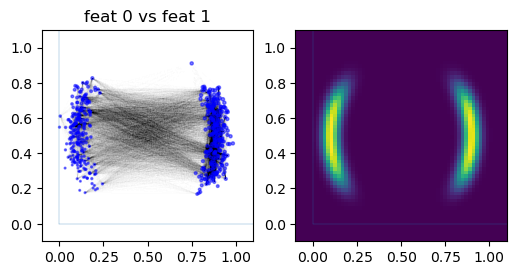
\includegraphics[width=\textwidth]{images/synthetic_2d/two_moons/moons_big_gt.png}    
        \end{minipage}  
        \caption{Right to left: ground truth synthetic prior and sampled graph. Top: graph sampled in $\mathcal{T}$ using PieClam. Bottom: graph sampled in $\mathbb{R}^2_+$ using Pclam.}
        \label{fig:ground truth 2d reconstruction}
\end{figure}

The optimization results are shown in Figures \ref{fig: unpriored models reconstruction} and \ref{fig: priored reconstructions}. Both the priored and unpriored models effectively learned the feature reconstructions in the feature spaces $\mathcal{T}$ and $\mathbb{R}_+^2$. Notably, the features in the priored models are more localized, supporting the claim that the prior acts as a regularizer.

The priors themselves are well-approximated, as illustrated in Figure \ref{fig: priored reconstructions}, with the quality of approximation improving as more nodes are sampled from the priors.


        
    % \item Priors have been reconstructed to a similar degree.%\pause
    % \item Shape also reconstructed with BigClam and IeClam.%\pause
    % \item Prior regularizes results.
    % \end{itemize}
    
\begin{figure}[t]
    \centering
    % Top row with small images
    \begin{minipage}{0.17\textwidth}
        \centering
        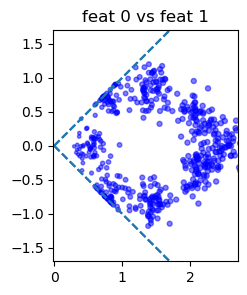
\includegraphics[width=\textwidth]{images/synthetic_2d/circle/circ_ie_reconstruct.png}
    \end{minipage}
    \hspace{0.02\textwidth}
    \begin{minipage}{0.2\textwidth}
        \centering
        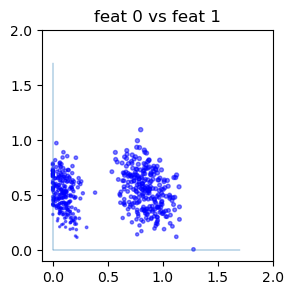
\includegraphics[width=\textwidth]{images/synthetic_2d/two_moons/moons_big_reconstruct.png}
    \end{minipage}
    \caption{Left to Right: IeClam and BigClam Reconstructions of features sampled from synthetic priors}
    \label{fig: unpriored models reconstruction}
\end{figure}
    % Bottom row with large images


\begin{figure}[t]
\centering
    \begin{minipage}{0.3\textwidth}
        \centering
        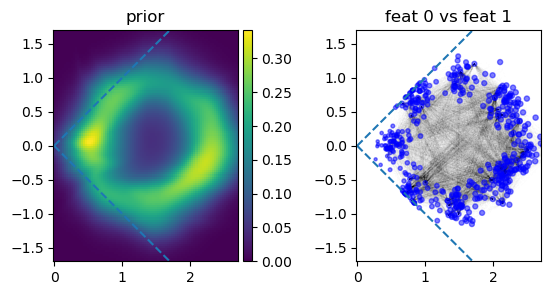
\includegraphics[width=\textwidth]{images/synthetic_2d/circle/pieclam_circ_reconstruct_edges.png}
    \end{minipage}
    
    \vspace{1em} % Add some vertical space between images
    \begin{minipage}{0.3\textwidth}
        \centering
        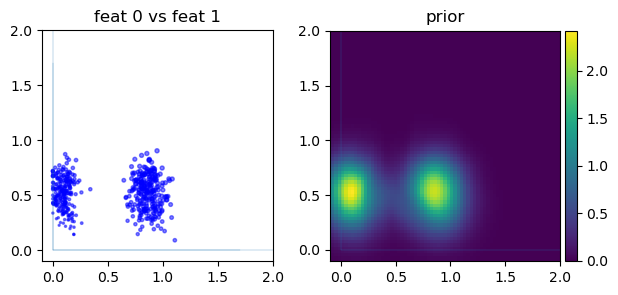
\includegraphics[width=\textwidth]{images/synthetic_2d/two_moons/moons_pclam_reconstructed.png}
    \end{minipage}
    \caption{Left to right: reconstructed nodes, reconstructed prior. Top to botton: PieClam in $\mathcal{T}$, PClam in $\mathbb{R_+^2}$}
    \label{fig: priored reconstructions}
\end{figure}

%\endgroup



\subsection{SBM Reconstruction And Distance Convergence}
We extend the experiment in Section \ref{sec:reconstruction_sbm} by considering another  synthetic SBM, which is off-diagonal dominant. As in Section \ref{sec:reconstruction_sbm}, we sample a simple graph with $N=210$ nodes from the SBM. The non zero probability blocks have a probability of $0.5$. We estimate the log cut distance between the Clam models (BigClam and IeClam) and the SBM during training. We consider for both methods affiliation spaces of dimensions $2,4$ and $6$. In addition, we calculate the cut distance and l2 errors between the Clam models and the SBM. The results are shown in Figures~\ref{fig:sbm_pclam1}--\ref{fig:sbm_pclam6}.



%BIGCLAM
\afterpage{
\begin{figure*}[!t]
    \begin{minipage}{0.5\columnwidth}

\includegraphics[width=0.8\textwidth]{images/sbm_reconstruction/halfdiag.png}       \end{minipage}\hfill  
\begin{minipage}{0.5\columnwidth}
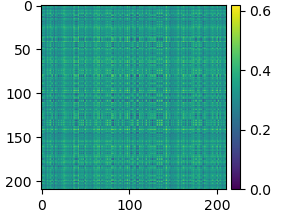
\includegraphics[width=0.8\textwidth]{images/sbm_reconstruction/halfdiag_bigclam/2_com/adj_cropped.png}       
\end{minipage}\hfill  
\begin{minipage}{1.1\columnwidth}
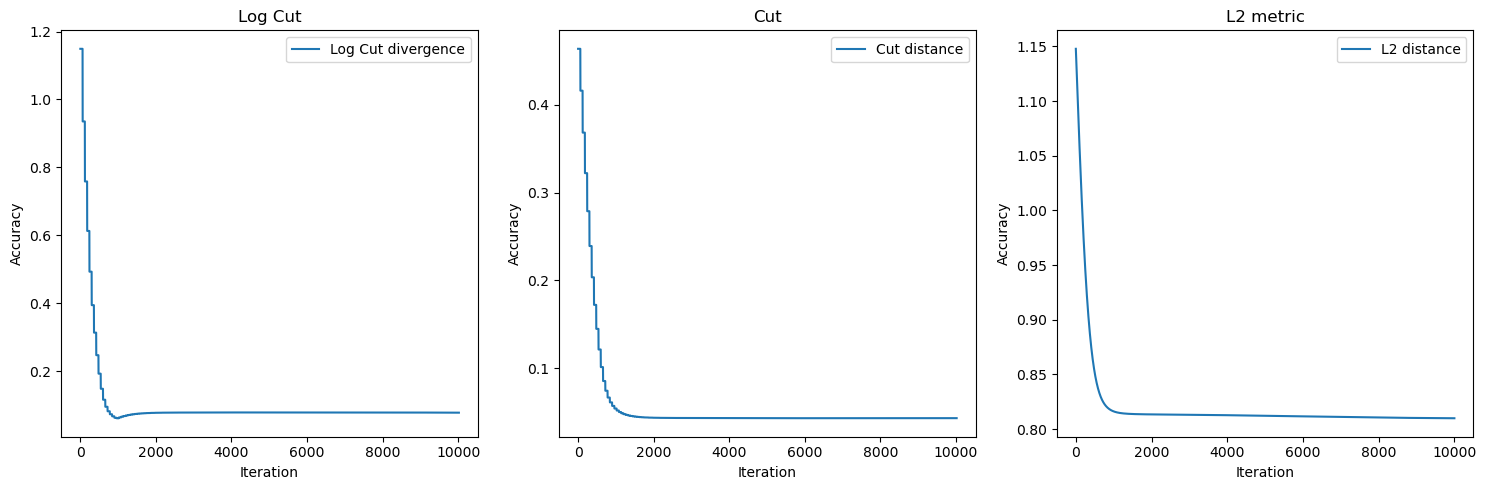
\includegraphics[width=0.8\textwidth]{images/sbm_reconstruction/halfdiag_bigclam/2_com/distances.png}
       \end{minipage}
    \caption{Left to right: Target SBM. Fitted BigClam graph with two communities. Error as a function of optimization iteration where error is, left to right,  log cut distance, cut distance, l2 distance. After convergence, the log cut distance between the SBM and BigClam is 0.0776.}
    \label{fig:sbm_pclam1}
\end{figure*}

\begin{figure*}[!t]
    \begin{minipage}{0.5\columnwidth}

\includegraphics[width=0.8\textwidth]{images/sbm_reconstruction/halfdiag.png}       \end{minipage}\hfill  
\begin{minipage}{0.5\columnwidth}

\includegraphics[width=0.8\textwidth]{images/sbm_reconstruction/halfdiag_bigclam/4_com/adj_cropped.png}       \end{minipage}\hfill  
\begin{minipage}{1.1\columnwidth}

\includegraphics[width=0.8\textwidth]{images/sbm_reconstruction/halfdiag_bigclam/4_com/distances.png}
       \end{minipage}
    \caption{Left to right: Target SBM. Fitted BigClam graph with four communities. Error as a function of optimization iteration where error is, left to right,  log cut distance, cut distance, l2 distance. After convergence, the log cut distance between the SBM and BigClam is 0.0775.}
    \label{fig:sbm_pclam2}
\end{figure*}

\begin{figure*}[!t]
    \begin{minipage}{0.5\columnwidth}

\includegraphics[width=0.8\textwidth]{images/sbm_reconstruction/halfdiag.png}       \end{minipage}\hfill  
\begin{minipage}{0.5\columnwidth}

\includegraphics[width=0.8\textwidth]{images/sbm_reconstruction/halfdiag_bigclam/6_com/adj_cropped.png}       \end{minipage}\hfill  
\begin{minipage}{1.1\columnwidth}

\includegraphics[width=0.8\textwidth]{images/sbm_reconstruction/halfdiag_bigclam/6_com/distances.png}
       \end{minipage}
    \caption{Left to right: Target SBM. Fitted BigClam graph with six communities. Error as a function of optimization iteration where error is, left to right,  log cut distance, cut distance, l2 distance. After convergence, the log cut distance between the SBM and BigClam is 0.0776.}
    \label{fig:sbm_pclam3}
\end{figure*}
% ====== bigclam =======

% IECLAM 

\begin{figure*}[!t]
    \begin{minipage}{0.5\columnwidth}

\includegraphics[width=0.8\textwidth]{images/sbm_reconstruction/halfdiag.png}       \end{minipage}\hfill  
\begin{minipage}{0.5\columnwidth}

\includegraphics[width=0.8\textwidth]{images/sbm_reconstruction/halfdiag_ieclam/2_com/adj_cropped.png}       \end{minipage}\hfill  
\begin{minipage}{1.1\columnwidth}
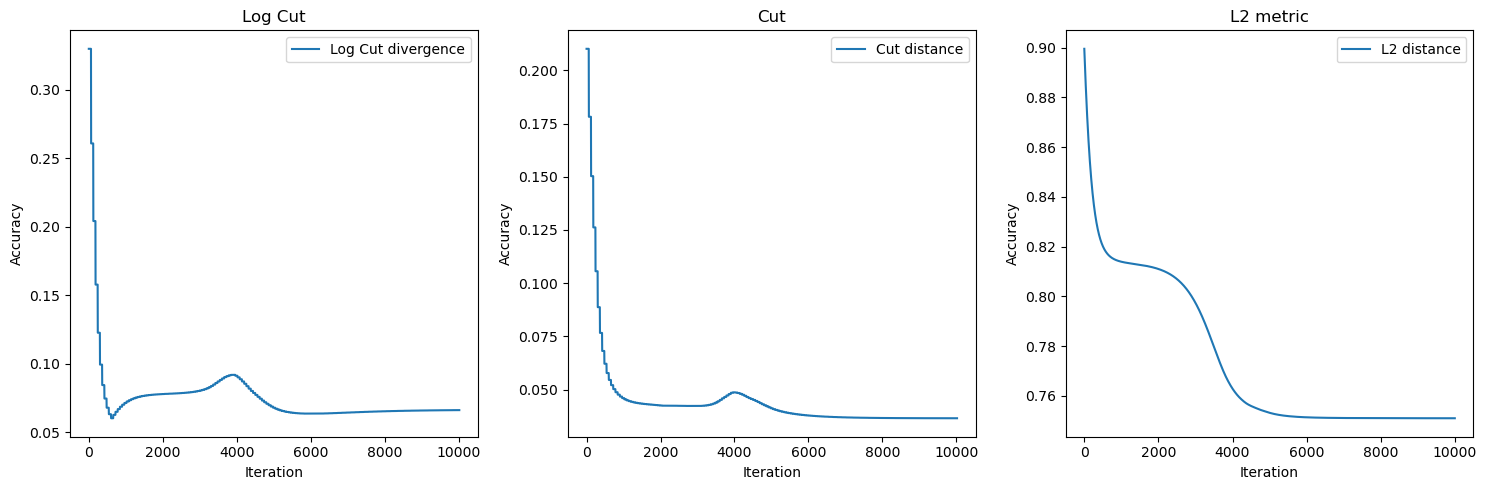
\includegraphics[width=0.8\textwidth]{images/sbm_reconstruction/halfdiag_ieclam/2_com/distances_2com.png}
       \end{minipage}
    \caption{Left to right: Target SBM. Fitted IeClam graph with two communities. Error as a function of optimization iteration where error is, left to right,  log cut distance, cut distance, l2 distance. After convergence, the log cut distance between the SBM and IeClam is 0.0662.}
    \label{fig:sbm_pclam4}
\end{figure*}

\begin{figure*}[!t]
    \begin{minipage}{0.5\columnwidth}

\includegraphics[width=0.8\textwidth]{images/sbm_reconstruction/halfdiag.png}       \end{minipage}\hfill  
\begin{minipage}{0.5\columnwidth}

\includegraphics[width=0.8\textwidth]{images/sbm_reconstruction/halfdiag_ieclam/4_com/adj_cropped.png}       \end{minipage}\hfill  
\begin{minipage}{1.1\columnwidth}
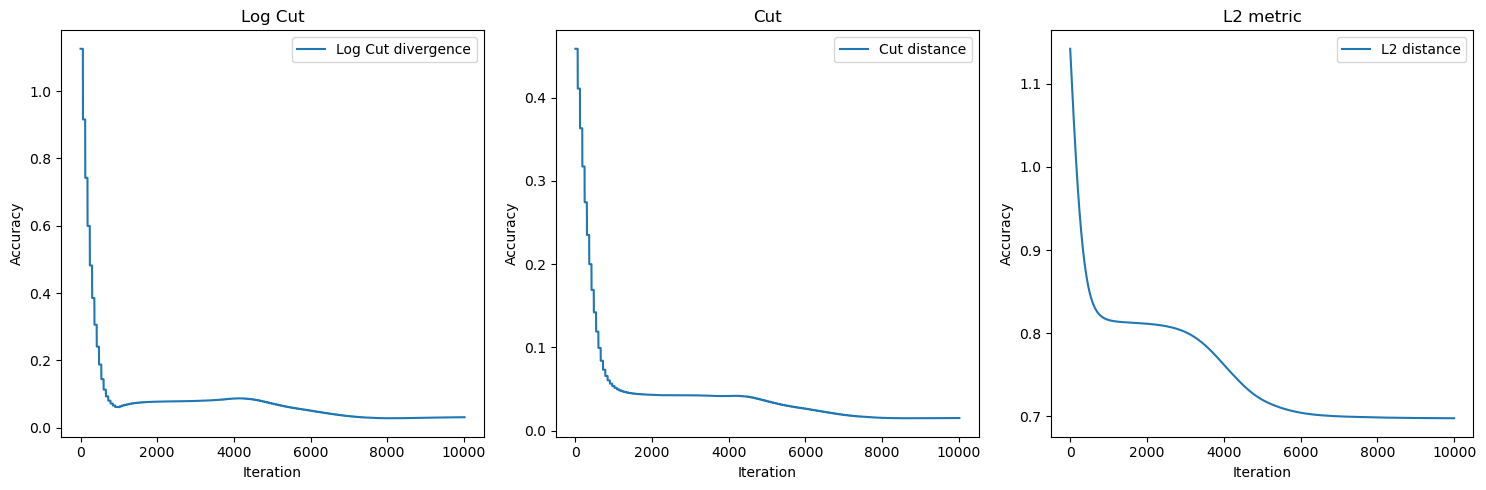
\includegraphics[width=0.8\textwidth]{images/sbm_reconstruction/halfdiag_ieclam/4_com/dists.png}
       \end{minipage}
    \caption{Left to right: Target SBM. Fitted IeClam graph with four communities (two inclusive and two exclusive). Error as a function of optimization iteration where error is, left to right,  log cut distance, cut distance, l2 distance. After convergence, the log cut distance between the SBM and IeClam is 0.0312.}
    \label{fig:sbm_pclam5}
\end{figure*}

\begin{figure*}[!t]
    \begin{minipage}{0.5\columnwidth}

\includegraphics[width=0.8\textwidth]{images/sbm_reconstruction/halfdiag.png}       \end{minipage}\hfill  
\begin{minipage}{0.5\columnwidth}

\includegraphics[width=0.8\textwidth]{images/sbm_reconstruction/halfdiag_ieclam/6_com/adj_cropped.png}       \end{minipage}\hfill  
\begin{minipage}{1.1\columnwidth}

\includegraphics[width=0.8\textwidth]{images/sbm_reconstruction/halfdiag_ieclam/6_com/distances.png}
       \end{minipage}
    \caption{Left to right: Target SBM. Fitted IeClam graph with six communities  (three inclusive and three exclusive). Error as a function of optimization iteration where error is, left to right,  log cut distance, cut distance, l2 distance. After convergence, the log cut distance between the SBM and IeClam is 0.0309.}
    \label{fig:sbm_pclam6}
\end{figure*}
}


%\begingroup
%\color{blue}
\subsection{Ablation Study}
\label{sec:ablation}
% \paragraph{Learning Rates and Number of Iterations.}
% A correct ratio between the learning rates and number of iterations of the prior and affiliation features is critical to the approximation's success. On one hand, if the features do not change enough in the $f$ iteration, 

% A learning rate on the prior that will be too large could collapse all of the features to one point. The learning rate of the features is affected both by the . The prior learning rate doesn't affect this velocity. instead, a learning rate of the prior that is too big will not give the nodes enough time to separate and will exert a pull on them that will make them eventually collapse to one point.

\paragraph{l$_1$ and $\mathbf{s}$ Regularization.}
The l$_1$ regularization is adapted from the BigClam original architecture and shows improvement when optimizing the models. This regularization type adds a constant update in all of the directions, which means that for every node $n$ and it's affiliation feature $\mathbf{f}_n$, components that are not updated are moved towards 0 regardless of their magnitude. This constant push towards 0 forces sparsity in the affiliation matrix and also acts as a regularization. The $\mathbf{s}$ regularization is an l$_1$ regularization of the $\mathbf{s}$ features and has shown effective for the Squirrel dataset.


\paragraph{Noise Addition.} Due to the high expressivity of the normalizing flow model, the neural network tends to learn a narrow distribution around the affiliation features. This overfitting tendency cannot be alleviated by simply reducing the network parameters without significantly compromising the expressivity of the prior. Noise addition offers a way to control the prior’s resolution while preserving its ability to learn complex distributions. An example comparing optimization results with and without noise addition is shown in Figure \ref{fig: noise comparison}.


\begin{figure}[t]
\centering
    \begin{minipage}{0.4\textwidth}
        \centering
        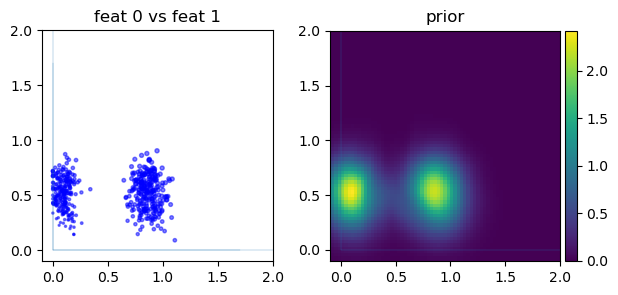
\includegraphics[width=\textwidth]{images/synthetic_2d/two_moons/moons_pclam_reconstructed.png}
    \end{minipage}
    
    \vspace{1em} % Add some vertical space between images
    \begin{minipage}{0.4\textwidth}
        \centering
        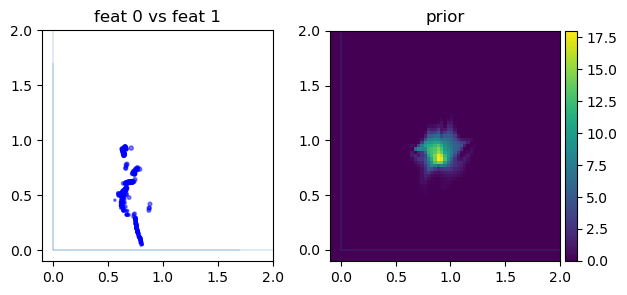
\includegraphics[width=\textwidth]{images/ablation/no_noise.png}
    \end{minipage}
    \caption{Left to right: reconstructed nodes, reconstructed prior. Top to botton: With and without noise addition.}
    \label{fig: noise comparison}
\end{figure}


\paragraph{Densification.}
\label{sec:ablation densification}
The densification method described in Section \ref{sec: densification definition} can yield varying results depending on the internal structure of the graph. To illustrate the impact of densification, we conducted 10 anomaly detection experiments, following the setup from Section \ref{sec:anomaly_detection}, but without applying densification. The results are shown in Table \ref{TableAblation}.
\begin{table}[H]
\centering
\small
\begin{tabular}{|c|c|c|c|}
    \hline
    Method & Reddit & Elliptic & Photo \\
    \hline
    (S) - PieClam & \textbf{64.12 ± 0.25} & 43.58 ± 0.15 & \underline{58.98 ± 2.51} \\
    (S) - PieClam (No Dens.) & 54.74 ± 0.13 & \textbf{40.02 ± 0.16} & 52.74 ± 0.71 \\
    \hline
    (P) - PieClam & 46.76 ± 2.50 & \textbf{63.18 ± 3.02} & 45.73 ± 7.03 \\
    (P) - PieClam (No Dens.) & 50.11 ± 4.24 & 64.11 ± 2.77 & 43.78 ± 0.78 \\
    \hline
    (PS) - PieClam & \textbf{63.99 ± 0.50} & 53.81 ± 1.63 & \textbf{58.99 ± 2.52} \\
    (PS) - PieClam (No Dens.) & 54.43 ± 0.68 & 62.29 ± 2.53 & 45.33 ± 0.47 \\
    \hline
\end{tabular}
% \begin{tabular}{|c|c|c|c|}
%     \hline
%   Method  & Reddit & Elliptic & Photo \\
%     \hline
%   (S) - PieClam & \textbf{0.6320 ± 0.0054} & \textbf{0.4354 ± 0.0005} & \textbf{0.5727 ± 0.0151} \\
%   (S) - PieClam (No Dens.) & 0.5480 ± 0.0022 & 0.4009 ± 0.0021& 0.5293 ± 0.0046\\
% \hline
%   (P) - PieClam & \underline{0.5089 ± 0.0219} & 0.6201 ± 0.0176 & \underline{0.4252 ± 0.0074} \\
%   (P) - PieClam (No Dens.) & \underline{0.5088 ± 0.0383}& \textbf{0.6378 ± 0.0245}& \underline{0.4325 ± 0.0089}\\
%     \hline
  
%   (PS) - PieClam & \textbf{0.6329 ± 0.0052} & 0.5294 ± 0.0089 & \textbf{0.5289 ± 0.0127} \\
%   (PS) - PieClam (No Dens,) & 0.5466 ± 0.0047& \textbf{0.6181 ± 0.0233}& 0.4538 ± 0.0030\\
%     \hline
% \end{tabular}
\caption{Comparison of PieClam on densified and non densified datasets. \textbf{Boldface} denotes a significantly better result (difference of over 2 standard deviations), \underline{underline} denotes an insignificant difference.}
\label{TableAblation}
\end{table}

As seen in Table \ref{TableAblation}, densification generally improved results across the datasets, except for the Elliptic dataset using the P and PS methods, where the undensified datasets performed significantly better. For the Reddit and Photo datasets with the P method, the difference was not significant.

% An open question for future work is identifying the conditions under which densification should be used. It is hypothesized that this decision may depend on the graph's homophily as defined in \cite{zhu2020graph_homophily}. In highly homophilic graphs, densification may preserve and strengthen community structures, whereas in bipartite or heterophilic structures, it may blur distinctions by overly connecting nodes within the same group. This is evident in Table \ref{TableAblation}, where densification improved anomaly detection on the homophilic Reddit and Photo graphs but worsened performance on the heterophilic Elliptic dataset.

%\endgroup
%%%%%%%%%%%%%%%%%%%%%%%%%%%%%%%%%%%%%%%%%%%%%%%%%%%%%%%%%%%%%%%%%%%%%%%%%%%%%%%
%%%%%%%%%%%%%%%%%%%%%%%%%%%%%%%%%%%%%%%%%%%%%%%%%%%%%%%%%%%%%%%%%%%%%%%%%%%%%%%


\end{document}


% This document was modified from the file originally made available by
% Pat Langley and Andrea Danyluk for ICML-2K. This version was created
% by Iain Murray in 2018, and modified by Alexandre Bouchard in
% 2019 and 2021 and by Csaba Szepesvari, Gang Niu and Sivan Sabato in 2022.
% Modified again in 2023 and 2024 by Sivan Sabato and Jonathan Scarlett.
% Previous contributors include Dan Roy, Lise Getoor and Tobias
% Scheffer, which was slightly modified from the 2010 version by
% Thorsten Joachims & Johannes Fuernkranz, slightly modified from the
% 2009 version by Kiri Wagstaff and Sam Roweis's 2008 version, which is
% slightly modified from Prasad Tadepalli's 2007 version which is a
% lightly changed version of the previous year's version by Andrew
% Moore, which was in turn edited from those of Kristian Kersting and
% Codrina Lauth. Alex Smola contributed to the algorithmic style files.
